% !TeX root = RJwrapper.tex
\title{A Study in Reproducibility: The Congruent Matching Cells
Algorithm and cmcR package}
\author{by Joseph Zemmels, Susan VanderPlas, and Heike Hofmann}

\maketitle

\abstract{%
Scientific research is driven by our ability to use methods, procedures,
and materials from previous studies and further this research by adding
to it. As the need for computationally-intensive methods to analyze
large amounts of data grows, the criteria needed to achieve
reproducibility, specifically computational reproducibility, have become
more sophisticated. In general, prosaic descriptions of algorithms are
not detailed or precise enough to ensure complete reproducibility of a
method. Results may be sensitive to conditions not commonly specified in
written-word descriptions such as implicit parameter settings or the
programming language used. To achieve true computational
reproducibility, it is necessary to provide all intermediate data and
code used to produce published results. In this paper, we consider a
class of algorithms developed at the National Institute of Standards and
Technology (NIST) to perform firearm evidence identification on
cartridge case evidence known as the \dfn{Congruent Matching Cells}
(CMC) methods. To date, only textual descriptions of these algorithms
have been published. We introduce the first open-source implementation
of the Congruent Matching Cells methods in the R package \CRANpkg{cmcR}.
We have structured the \CRANpkg{cmcR} package as a set of sequential,
modularized functions intended to ease the process of parameter
experimentation. We use \CRANpkg{cmcR} and a novel variance ratio
statistic to explore the CMC methodology and illustrate problems that
arise when computationally ambiguous algorithms descriptions are
provided.
}

\defcitealias{pcast}{PCAST,~2016}
\defcitealias{daubert}{Daubert~v.~Merrel~Dow~Pharmaceuticals,~Inc.}

\hypertarget{intro}{%
\section{Introduction}\label{intro}}

Forensic examinations are intended to provide an objective assessment of
the probative value of a piece of evidence. Typically, this assessment
of probative value is performed by a forensic examiner who visually
inspects the evidence to determine whether it matches evidence found on
a suspect. The process by which an examiner arrives at their evidentiary
conclusion is largely opaque and has been criticized \citepalias{pcast}
because its' subjectivity does not allow for an estimation of error
rates. In response, \citet{council_strengthening_2009} pushed to augment
subjective decisions made by forensic examiners with automatic
algorithms that objectively assess evidence and can be explained during
court testimony. In addition to the objectivity of these algorithms,
there is an additional benefit: we expect that an algorithm run on the
same data multiple times will produce the same answer; that is, that the
results are repeatable. This is extremely beneficial because it allows
the prosecution and defense to come to the same conclusion given
objective evidence or data.

\hypertarget{repeatability-and-reproducibility}{%
\subsection{Repeatability and
Reproducibility}\label{repeatability-and-reproducibility}}

Repeatability in forensic labs is enforced primarily using standard
operating procedures (SOPs), which specify the steps taken for any given
evaluation, along with the concentrations of any chemicals used, the
range of acceptable machine settings, and any calibration procedures
required to be completed before the evidence is evaluated. When labs use
computational procedures, this SOP is augmented with specific
algorithms, which are themselves SOPs intended for use by man and
machine. Algorithms are generally described on two levels: we need both
the conceptual description (intended for the human using the algorithm)
and the procedural definition (which provides the computer hardware with
a precise set of instructions).\} For scientific and forensic
repeatability and reproducibility, it is essential to have both pieces:
the algorithm description is critical for establishing human
understanding and justifying the method's use in court, but no less
important is the computer code which provides the higher degree of
precision necessary to ensure the results obtained are similar no matter
who evaluates the evidence. As with SOPs in lab settings, the code
parameters function like specific chemical concentrations; without those
details, the SOP would be incomplete and the results produced would be
too variable to be accepted in court.

\citet{nas_2019} defines \dfn{reproducibility} as ``obtaining consistent
computational results using the same input data, computational steps,
methods, code, and conditions of analysis.'' This form of
reproducibility requires that the input data, code, method, and
computational environment are all described and made available to the
community. Obviously, in many situations, this level of reproducibility
is not provided. There are only a few open-source pattern-matching
algorithms in forensics (glass \citep{park2019}, handwriting
\citep{crawford_handwriting_2020}, shoe prints
\citep{park_algorithm_2020}, and ballistic evidence
\citep{hare_automatic_2016,tai_fully_2018}); the vast majority of
proposed methods do not adhere to the definition of reproducibility in
\citet{nas_2019}.

Instead, we find it useful to consider a more inclusive hierarchy of
reproducibility.

\begin{definition} Hierarchy of Reproducibility \label{reprod-defn}

\begin{description}
\item[Conceptual description] The algorithm is described and demonstrated in a scientific publication.
\item[Pseudocode] The algorithm is described at a high level of detail with pseudocode implementation provided, and is demonstrated in a scientific publication
\item[Reproducible data] The algorithm is described and demonstrated in a scientific publication, and input data are available in supplementary material.
\item[Comparable results] The algorithm is described and demonstrated in a scientific publication, and input data and numerical results are provided in supplementary material.
\item[Full reproducibility] The algorithm is described and demonstrated in a scientific publication, and the input data, source code, parameter settings, and numerical results are provided in supplementary material.
\end{description}
\end{definition}

To aid in comprehension of an algorithm, it is useful to supplement
conceptual descriptions with pseudocode. However, a conceptual
description and pseudocode alone do not contain sufficient detail (e.g.,
parameter settings) to ensure computational reproducibility. Commonly
identified reasons for unreproducible results include (1) ambiguity in
how procedures were implemented, (2) missing or incomplete data, and (3)
missing or incomplete computer code to replicate all statistical
analyses \citep{leek_is_2017}. In particular, for statistical algorithms
which depend on input data, we find that full reproducibility depends on
the provision of both original data and any manual preprocessing applied
to said data, as this manual process is not reproducible by itself. In
combination with the code, the algorithm description, and the numerical
results presented in the paper, it should be possible to fully reproduce
the results of a paper.

In this paper, we demonstrate the importance of higher levels of
reproducibility by examining the Congruent Matching Cells (CMC)
algorithm for cartridge case comparisons and developing an open-source,
fully reproducible version for general use in the forensics community.

\hypertarget{the-congruent-matching-cells-algorithm}{%
\subsection{The Congruent Matching Cells
Algorithm}\label{the-congruent-matching-cells-algorithm}}

A \dfn{cartridge case} is the portion of firearm ammunition that encases
a projectile (e.g., bullet, shots, or slug) along with the explosive
used to propel the projectile through the firearm. When a firearm is
discharged, the projectile is propelled down the barrel of the firearm,
while the cartridge case is forced towards the back of the barrel. It
strikes the back wall, known as the \dfn{breech face}, of the barrel
with considerable force, thereby imprinting any markings on the breech
face onto the cartridge case and creating the so-called
\dfn{breech face impressions}. These markings have been suggested to be
unique to a firearm and are used in forensic examinations to determine
whether two cartridge cases have been fired by the same firearm. During
a forensic examination, two pieces of ballistic evidence are placed
under a \dfn{comparison microscope}. Comparison microscopes allow for a
side-by-side comparison of two objects within the same viewfinder, as
seen in \autoref{fig:ccPair_combined}. A pair of breech face images is
aligned along the thin black line in the middle of the images. The
degree to which these breech face markings can be aligned is used to
determine whether the two cartridge cases came from the same source;
i.e., were fired from the same firearm. These breech face impressions
are considered to be a firearm's unique ``fingerprint'' left on a
cartridge case \citep{firearm_id_thompson}.

\begin{Schunk}
\begin{figure}[htbp]
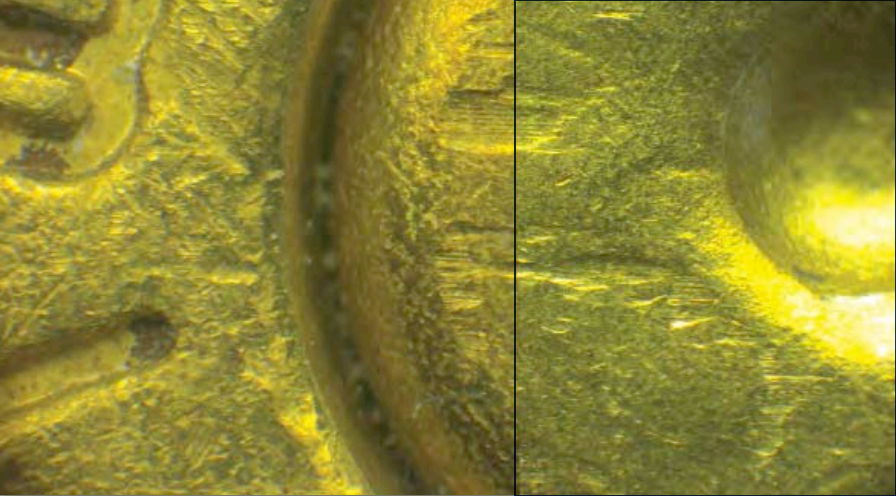
\includegraphics[width=\textwidth]{images/cartridgeCasePair_comparison_with_line} \caption{\label{fig:ccPair_combined} A cartridge case pair with visible breech face impressions under a microscrope.  A thin line can be seen separating the two views. The degree to which the markings coincide is used to conclude whether the pair comes from the same source.}\label{fig:unnamed-chunk-1}
\end{figure}
\end{Schunk}

The Congruent Matching Cells (CMC) pipeline is a collection of
algorithms developed at the National Institute of Standards and
Technology (NIST) in 2012 to process and compare cartridge case evidence
\citep{song_proposed_2013}. Since then, the pipeline and its numerous
extensions
\citep{tong_improved_2015,chen_convergence_2017,song_estimating_2018}
have shown promise in being able to differentiate between matching and
non-matching cartridge cases. However, so far the CMC pipelines have
only been introduced conceptually in the form of written-word
descriptions. Further, the cartridge case scans used to validate the
pipelines are only available in their raw, unprocessed forms on the NIST
Ballistics Research Database \citep{nbtrd}. While it is clear that the
creators of the CMC pipeline have a working implementation, the wider
forensic science community only has access to conceptual descriptions of
the pipeline and some summary statistics describing its performance.

Here, we describe the process of implementing the CMC pipeline for the
comparison of marks on spent cartridge cases, using the descriptions
from two published papers, \citet{song_3d_2014} and
\citet{tong_improved_2015}. Our R package, \CRANpkg{cmcR}, provides an
open-source implementation of the CMC pipeline. We use \CRANpkg{cmcR} to
illustrate how ambiguities in the textual description of an algorithm
can lead to highly divergent results. In particular, our implementation
highlights an extreme sensitivity to processing and parameter decisions
that has not been discussed previously. Additionally, we argue that our
implementation can be used as a template for future implementations of
forensic pattern-matching algorithms to not only ensure transparency and
auditability, but also to ease experimentation and improvement.

In the remainder of this paper, we describe a general, reproducible, and
open-source CMC pipeline which encompasses those discussed in
\citet{song_proposed_2013}, \citet{song_3d_2014}, and
\citet{tong_improved_2015}. \citet{song_proposed_2013} lays out the
conceptual framework for the original CMC pipeline later implemented in
\citet{song_3d_2014} and \citet{tong_fired_2014}. An improvement of the
pipeline presented in \citet{tong_improved_2015} and used in subsequent
papers is referred to as the ``High CMC" method
\citep{chen_convergence_2017}. However, it should be noted that what the
authors refer to as the original and High CMC decision rules are
variations of one step of a larger CMC pipeline.

Both decision rules (and other proposed variations\}) have been shown to
correctly differentiate same and different-source cartridge cases from
the \citet{fadul_empirical_2011} data set. The \CRANpkg{cmcR} package
contains implementations designed for use with 3D topographical scans of
the original decision rule described in \citet{song_proposed_2013} and
\citet{song_3d_2014} and the High CMC decision rule described in
\citet{tong_improved_2015}. The source code to the full \CRANpkg{cmcR}
package is accessible at \url{https://github.com/CSAFE-ISU/cmcR}.

\hypertarget{cmcMethod}{%
\section{The CMC pipeline}\label{cmcMethod}}

In this section, we examine the process of implementing the CMC pipeline
for automatic comparisons of 3D cartridge case scans. At each step, we
will compare the description in the published papers with the
implementation in code, discussing the gaps in the pipeline description
and how we filled in those gaps during the creation of \CRANpkg{cmcR}.
We discuss each stage of the CMC pipeline using excerpts from the
original papers. Then, we examine the implementation of each
sub-procedure in the \CRANpkg{cmcR} package, considering the differences
between the textual description and its algorithmic translation.

All of the CMC pipelines can be broken down into three broad stages: (1)
preprocessing, (2) cell-based similarity feature extraction, and (3)
application of a decision rule as illustrated in
\autoref{fig:overview-flow}. In the following sections we break each of
these stages further into a set of modular steps. One advantage of
modularizing these algorithms is that we can implement an algorithm as a
set of sequential procedures. This allows us to test new variations
against the old implementation in a coherent, unified framework.

\begin{figure}
\centering
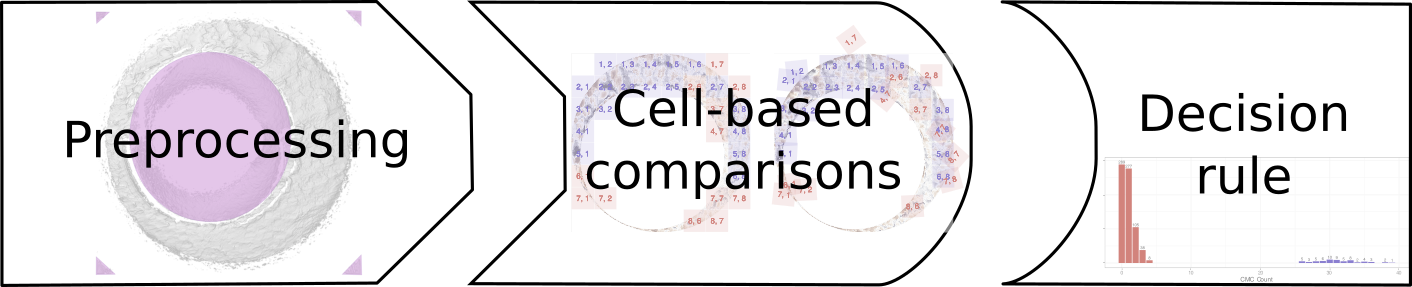
\includegraphics[width=.8\textwidth]{images/overview-flow.png}
\caption{The stages of CMC pipelines. In the preprocessing stage, each scan is prepared for analysis, removing extraneous information and noise. Then, each scan is broken up into cells, which are numerically compared to cells in the other scan to determine an optimal alignment. Finally, each of the scores arising from the cells in the second stage are compared to a reference distribution to determine whether the scans originate from the same source or from different sources.\label{fig:overview-flow}}
\end{figure}

The primary difference between the two pipelines presented here, the
original and High CMC decision rules, lies in how the decision rules are
utilized to separate matches and non-matches. Beyond that there are also
several small differences in the parameters used in the preprocessing
and comparison procedures. Despite using the same validation data from
\citet{fadul_empirical_2011} across papers, current authors do not
provide justification for changing these parameters. At the same time,
different conditions have been shown to yield very different results;
even when applying the same decision rule. This sensitivity of various
pipelines to different conditions has not previously been discussed in
detail.

\hypertarget{initialData}{%
\subsection{Initial Data}\label{initialData}}

Digital microscopy is capable of precision measurements of surface
topology at even higher resolutions. Using a 3D microscope, we can
obtain scans of breech face impressions at the micron level
(\(1 \mu m = 10^{-3} mm = 10^{-6} m\)). These 3D topological scans are
used as input to automated comparison algorithms, such as the CMC
pipeline originally proposed in \citet{song_proposed_2013}. We will use
the same data set which is referenced in \citet{song_3d_2014} and
\citet{tong_improved_2015} to illustrate usage of the \CRANpkg{cmcR}
package. These 3D scans of cartridge cases are available from the NIST
Ballistics Toolmark Research Database \citep[NBTRD;][]{nbtrd}. The
strings defined below refer to three cartridge case scans available on
the NBTRD from \citet{fadul_empirical_2011} and will be used throughout
the remainder of this paper.

\begin{Schunk}
\begin{Sinput}
library(cmcR)

nbtrd_url <- "https://tsapps.nist.gov/NRBTD/Studies/CartridgeMeasurement"

x3p_ids <- c("DownloadMeasurement/2d9cc51f-6f66-40a0-973a-a9292dbee36d",
             "DownloadMeasurement/cb296c98-39f5-46eb-abff-320a2f5568e8",
             "DownloadMeasurement/8ae0b86d-210a-41fd-ad75-8212f9522f96")

file_names <- c("fadul1-1.x3p","fadul1-2.x3p","fadul2-1.x3p")

purrr::walk2(.x = x3p_ids,
             .y = file_names,
             .f = function(x3p_id,file_name){
               download.file(url = file.path(nbtrd_url, x3p_id),
                             destfile = paste0("data/",file_name),mode = "wb")
             })
\end{Sinput}
\end{Schunk}

Cartridge case scans are commonly stored in the ISO standard x3p file
format \citep{ISO25178-72}. x3p is a container format which consists of
a single surface matrix representing the height value of the breech face
surface and metadata concerning the parameters under which the scan was
taken (size, resolution, creator, microscope, and microscopy software
versions etc.). The \CRANpkg{x3ptools} package \citep{x3ptools} provides
functionality to work with the format in R.

\autoref{fig:cartridgeCasePair} shows the surface matrices of a known
match (KM) pair of cartridge cases from a study by
\citet{fadul_empirical_2011}. In this study, a total of 40 cartridge
cases were scanned with a lateral resolution of 6.25 microns
(micrometers) per pixel. The surface matrices are approximately
\(1200 \times 1200\) pixels in size corresponding to an area of about
\(3.8 \times 3.8\) mm\(^2\).

\begin{Schunk}
\begin{figure}[htbp]

{\centering \subfloat[\label{fig:rawBFs-1}]{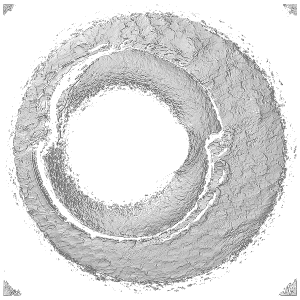
\includegraphics[width=.49\linewidth,height=.49\linewidth]{figures/fadul1-1} }\subfloat[\label{fig:rawBFs-2}]{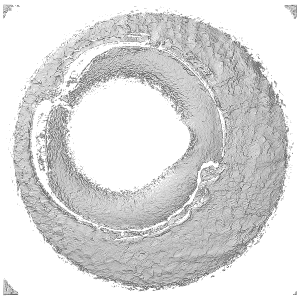
\includegraphics[width=.49\linewidth,height=.49\linewidth]{figures/fadul1-2} }

}

\caption{\label{fig:cartridgeCasePair} Unprocessed surface matrices of the known-match Fadul 1-1 (left) and Fadul 1-2 (right) \citep{fadul_empirical_2011}. The observations in the corners of these surface matrices are artifacts of the staging area in which these scans were taken. The holes on the interior of the primer surfaces are caused by the firing pin striking the primer during the firing process. The region of the primer around this hole does not come into uniform contact with the breech face of the firearm.}\label{fig:rawBFs}
\end{figure}
\end{Schunk}

Only certain regions of a cartridge case contain identifying breech face
impression markings. \citet{song_proposed_2013} defines ``valid
correlation regions'' as regions where ``the individual characteristics
of the ballistics signature are found that can be used effectively for
ballistics identification.'' Prior to applying the CMC comparison
procedure, cartridge scans must undergo some preprocessing to identify
these valid correlation regions.

\hypertarget{preProcessing}{%
\subsection{Preprocessing procedures}\label{preProcessing}}

During the preprocessing stage, a series of sequential steps is used to
prepare each cartridge case for analysis. The goal of this process is to
remove the edges and center of the scan which did not come into contact
with the breech face, as well as any artifacts of the scan and
microscope staging which do not accurately represent the breech face
surface.

The different iterations of the CMC algorithm describe different
variations of these steps. A summary of these steps is shown in
\autoref{fig:preprocessing-schematic}.

\begin{figure}
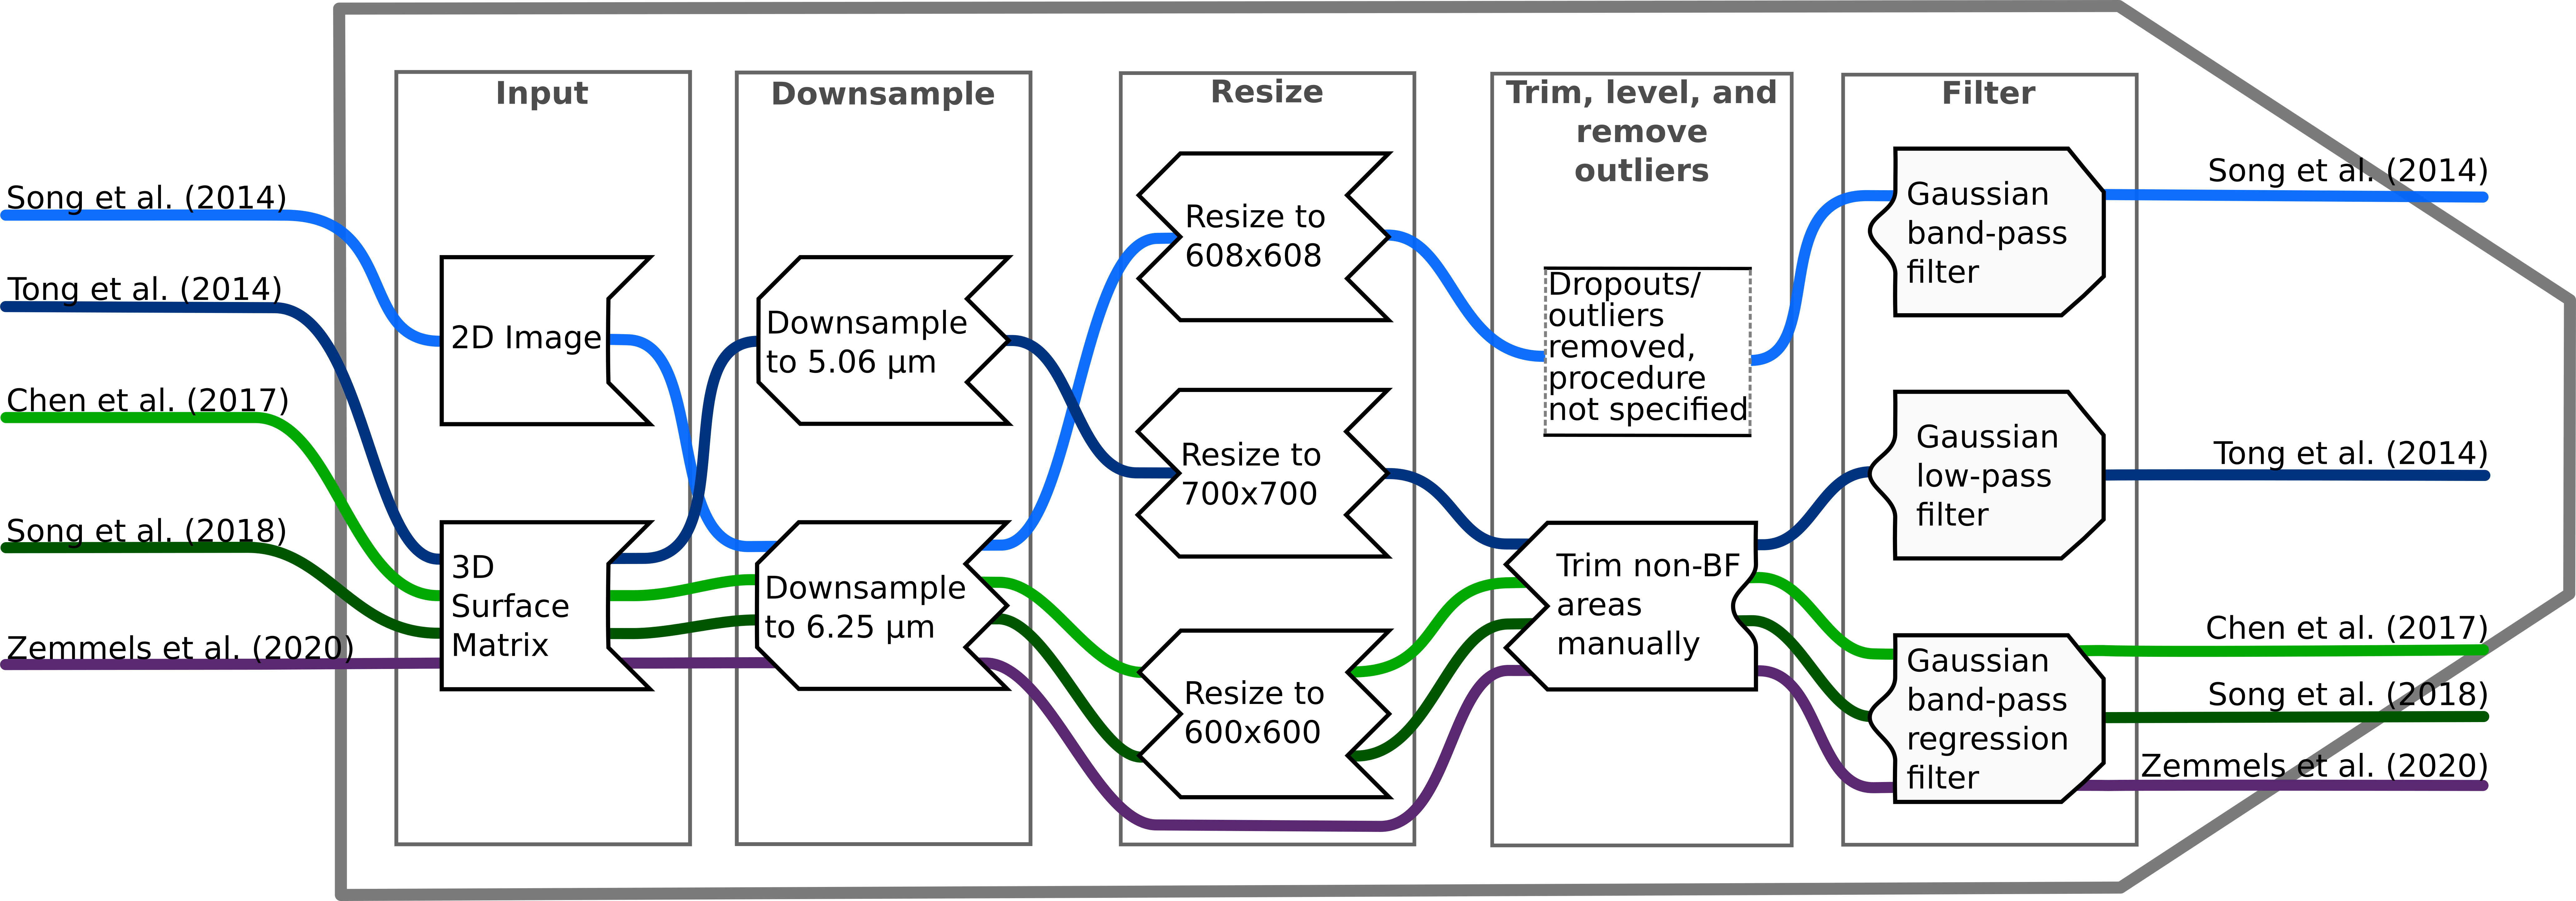
\includegraphics[width=\linewidth]{images/preprocessing_flow.png}
\caption{Overview of the set of pre-processing steps used in the CMC algorithms. Where a procedure step is not discussed or explicitly not applied in the paper, the path traverses empty space.}\label{fig:preprocessing-schematic}
\end{figure}

The implementation in \citet{tong_fired_2014} describes the
preprocessing steps (for the 2D images) as:

\begin{quote}
After trimming processing {[}sic{]} to remove unrelated correlations
areas, the final image size is reduced to 700 × 700 pixel with an
estimated pixel spacing of 5.0 \(\mu\)m. A Gaussian smoothing filter
(standard deviation \(\sigma\) = 1) was implemented first to remove high
frequency noise.
\end{quote}

\citet{song_3d_2014} outline the following preprocessing procedure on 3D
scans:

\begin{quote}
Trim off the inside firing pin surface and other areas outside the
breech face mark, so that only breech face impression data remain for
correlation.
\end{quote}

\begin{quote}
Identify and remove dropouts or outliers.
\end{quote}

\begin{quote}
Apply a band-pass Gaussian regression filter with 40 \(\mu\)m short
cutoff length and 400 \(\mu\)m long cutoff length to remove low
frequency components, including surface curvature, form error, waviness
and high frequency components which mainly arise from the instrument
noise.
\end{quote}

While not explicitly mentioned in \citet{song_3d_2014},
\citet{song_estimating_2018} indicates that the ``trimming'' of the
unwanted regions of the scan is performed manually. No further
information is given in the paper describing what criteria were used for
this process; nor are the trimmed scans provided as intermediate data
for the sake of reproducibility.

It is also unclear how the dropouts and outliers are ``removed'' from
the scan or even how outliers are defined; many different methods for
outlier detection and removal are used in surface metrology
\citep{outlierdetection}. Most of these algorithms require the user to
select thresholds or parameters; thus, without any details about how the
outlier detection process was implemented, this portion of
\citet{song_3d_2014} is not reproducible.

We are not aware of an open-source implementation of the multivariate
band-pass Gaussian regression filter used in surface metrology
\citep{ISO16610-71}. Further, there are various parameters requiring
specification to implement a Gaussian regression filter and it is not
clear how these parameters were chosen
\citep{brinkman_bodschwinna_2003}.

As a result of these ambiguities, during our implementation of the
preprocessing algorithm, we had to make several educated guesses in
order to match the described procedure (and reported results) as closely
as possible.

\hypertarget{implementation-of-preprocessing-procedures}{%
\subsubsection{Implementation of preprocessing
procedures}\label{implementation-of-preprocessing-procedures}}

The preprocessing procedures are implemented via modularized functions
of the form \code{preProcess\_*}. Modularizing the steps of the
preprocessing procedures makes the overall process easier to understand
and allows for experimentation. \autoref{fig:processingPipeline} shows
an overview of the preprocessing framework for the Fadul 1-1 breech face
from reading the scan (left) to an analysis-ready region (right). For
each scan in \autoref{fig:processingPipeline}, eleven height value
percentiles: the Minimum (0th), 1st, 2.5th, 10th, 25th, Median (50th),
75th, 90th, 97.5th, 99th, and Maximum (100th) are mapped to a
purple-to-orange color gradient. This mapping is chosen to highlight the
extreme values in each scan.

\begin{Schunk}
\begin{figure}[htbp]

{\centering 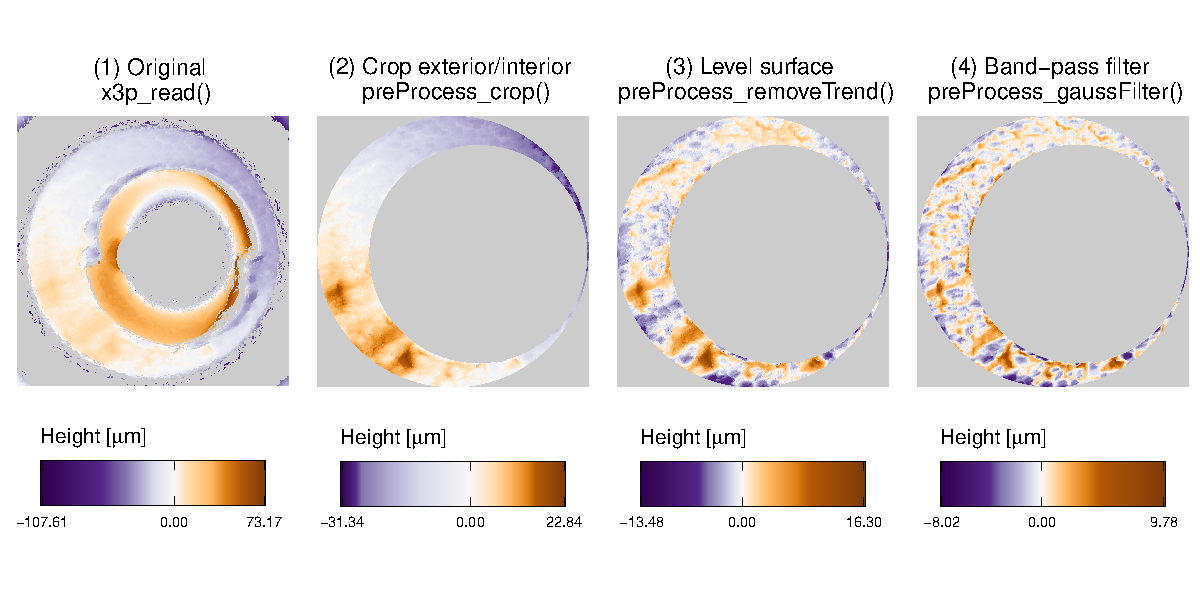
\includegraphics[width=\textwidth]{figures/cmcr-unnamed-chunk-5-1} 

}

\caption{\label{fig:processingPipeline} Illustration of the  preprocessing pipeline implemented in \CRANpkg{cmcR}.  At each stage, the variability in height across the scan decreases as extraneous sources of noise are removed.}\label{fig:unnamed-chunk-5}
\end{figure}
\end{Schunk}

We demonstrate usage of the \code{preProcess\_*} functions on the Fadul
1-1 scan. Each code chunk is followed up with an explanation of the
functions used.

\begin{Schunk}
\begin{Sinput}
# Step (1)
fadul1.1 <- x3ptools::x3p_read("data/fadul1-1.x3p")
\end{Sinput}
\end{Schunk}

We begin with a 3D scan. Typically, scans are downsampled to about 25\%
of their size by only retaining every other row and column in the
surface matrix. The breech faces in \citet{fadul_empirical_2011} were
initially scanned at a resolution of 3.125 \(\mu\)m per pixel.
Downsampling reduces the resolution to 6.25 \(\mu\)m per pixel. Step (1)
in \autoref{fig:processingPipeline} shows an unprocessed breech face
scan.

\begin{Schunk}
\begin{Sinput}
# Step (2)
fadul1.1_cropped <- fadul1.1 %>%
  cmcR::preProcess_crop(region = "exterior") %>%
  cmcR::preProcess_crop(region = "interior")
\end{Sinput}
\end{Schunk}

Three major regions of the scan are identified via a labeling algorithm
as described in \citet{hesselink_concurrent_2001} and available in the
\CRANpkg{imager} package \citep{imager}. These regions are the circle
capturing the exterior of the cartridge case primer, the breech face
impression region, and the circle around the firing pin impression hole
in the center of the scan.

The goal is to isolate the breech face impression region by removing
(i.e., replacing with \code{NA}) the pixels in the other two regions.
Upon labeling the different regions of the cartridge case scan, the
centers and radii of the cartridge case primer and firing pin impression
hole are estimated. This estimation procedure may require some user
input depending on how much of the exterior/interior the user wants
removed. The resulting breech face scan, like the one shown in step (2)
of \autoref{fig:processingPipeline}, is reproducible assuming the same
user-specified settings are used. The \code{preProcess\_crop} function
removes the exterior and firing pin impression region on the interior
based on the \code{region} argument.

\begin{Schunk}
\begin{Sinput}
# Step (3)
fadul1.1_deTrended <- fadul1.1_cropped %>%
  preProcess_removeTrend(statistic = "quantile", tau = .5, method = "fn")
\end{Sinput}
\end{Schunk}

In step (3) any existing large-scale trend in the breech face scan
height values are removed. In steps (1) and (2) of
\autoref{fig:processingPipeline} it is clear that there is a
southwest-to-northeast trend in height values. Such a trend is
observable in many cartridge case scans, yet does not occur consistently
across cartridge cases fired from the same firearm. This indicates that
a trend in height values is likely to be an artifact of the scanning
process resulting from cartridge cases not being precisely, horizontally
leveled prior to taking the scan. Neglecting to remove these trends
leads to very different results based on our implementation. In an
extreme situation, two different-source cartridge cases with similar
trends might be incorrectly deemed ``congruent.'' The
\code{preProcess\_removeTrend} functions levels the breech face
impression regions obtained from step (2). The function estimates and
subtracts the conditional median via a quantile regression as
implemented in the \code{rq} function of the \CRANpkg{quantreg} package
\citep{quantreg}. Step (3) of \autoref{fig:processingPipeline} shows a
median-leveled breech face scan.

\begin{Schunk}
\begin{Sinput}
# Step (4)
fadul1.1_processed <- fadul1.1_deTrended %>%
  preProcess_gaussFilter(filtertype = "bp", wavelength = c(16,500)) %>%
  x3ptools::x3p_sample(m = 2)
\end{Sinput}
\end{Schunk}

In the final preprocessing step, a band-pass filter is applied to the
processed breech face scan to reduce the effects of undesired
frequencies in the comparison procedure. For example, low frequency
(large wavelength) global structure may exist in a cartridge case scan
due to manufacturing specifications. In forensics, this type of
structure is referred to as a class or subclass characteristic -- it is
shared by many objects of the same make and model. Class characteristics
are used by forensic practitioners to initially pare down the possible
pool of matching cartridge cases \citep{firearm_id_thompson}. While this
additional global structure may assist with matching cartridge cases, it
can also artificially inflate the similarity between truly non-matching
scans. The goal of comparing breech-face scans is to answer the question
of source. Same-sourceness can only be determined by matching individual
characteristics, so the global structure is removed by using a high-pass
Gaussian filter. Similarly, a low-pass filter is used to remove noise
and outliers from cartridge case scans due to, for example,
imperfections in the scanning process. A band-pass Gaussian filter
combines the effects of low and high-pass filters; this is the default
choice in \CRANpkg{cmcR}. The band-pass filtered breech face scan as
returned by the \code{preProcess\_gaussFilter} function is shown in the
fourth panel of \autoref{fig:processingPipeline}.

There is currently no determination or removal of outliers in the
\CRANpkg{cmcR} package's preprocessing procedures. Instead, we rely on
the low-pass portion of the Gaussian filter to reduce the effects of any
high-frequency noise.

\autoref{fig:processedScans} displays the processed Fadul 1-1 and Fadul
1-2 scans; the second matrix is processed using the same parameters.
Similarity features are extracted from a processed cartridge case pair
in the cell-based comparison procedure.

\begin{Schunk}
\begin{figure}[htbp]

{\centering 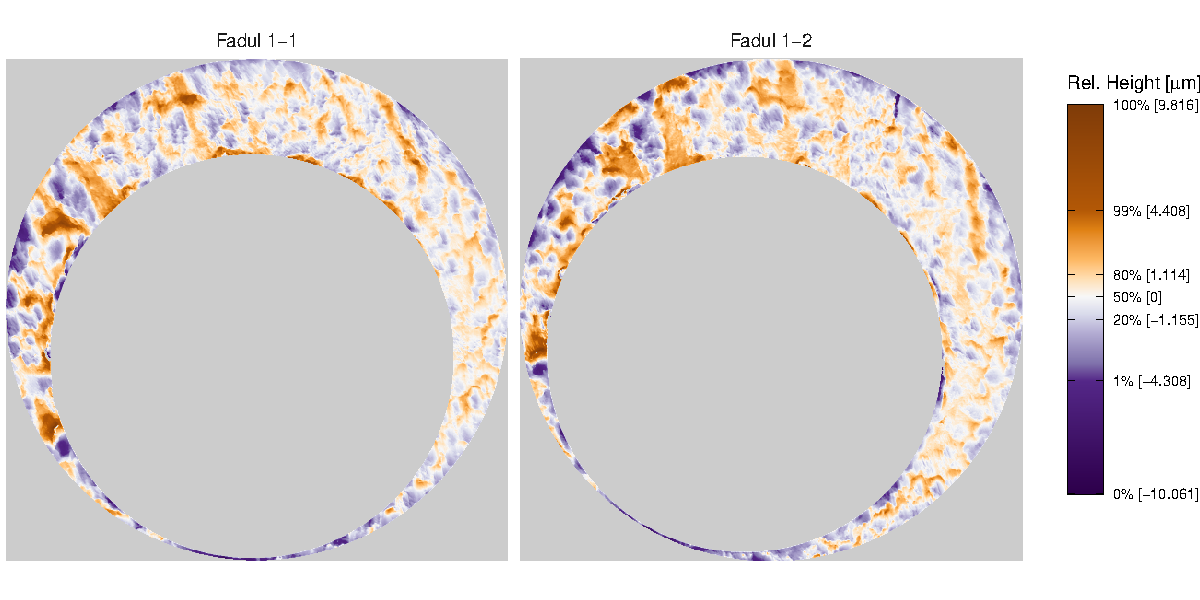
\includegraphics[width=\textwidth]{figures/cmcr-unnamed-chunk-10-1} 

}

\caption{\label{fig:processedScans} Fadul 1-1 and Fadul 1-2 after preprocessing. Similar striated markings are now easier to visually identify on both surfaces. It is now clearer that one of the scans needs to be rotated to align better with the other.}\label{fig:unnamed-chunk-10}
\end{figure}
\end{Schunk}

\hypertarget{comparisonProcedure}{%
\subsection{``Correlation cell'' comparison
procedure}\label{comparisonProcedure}}

As described in \citet{song_proposed_2013}, breech face markings are not
uniformly impressed upon a cartridge case during the firing process. As
such, only certain sections of the cartridge case are used in a
comparison. In the CMC pipeline as proposed by
\citet{song_proposed_2013} two scans are compared by partitioning one
breech face scan into a grid of so-called ``correlation cells''. These
cells are compared individually to their best-matching counterpart on
the other scan. If a large proportion of these correlation cells are
highly similar to their counterparts on the other breech face scan, this
is considered as evidence that the markings on the two cartridge cases
were made by the same source. The number of highly similar cells is
defined as the \dfn{CMC count} \(C\) \citep{song_proposed_2013} of the
breech-face comparison. The CMC count is considered to be a more robust
similarity metric than a cross-correlation score based on the entire
cartridge case.

\begin{Schunk}
\begin{figure}[htbp]

{\centering 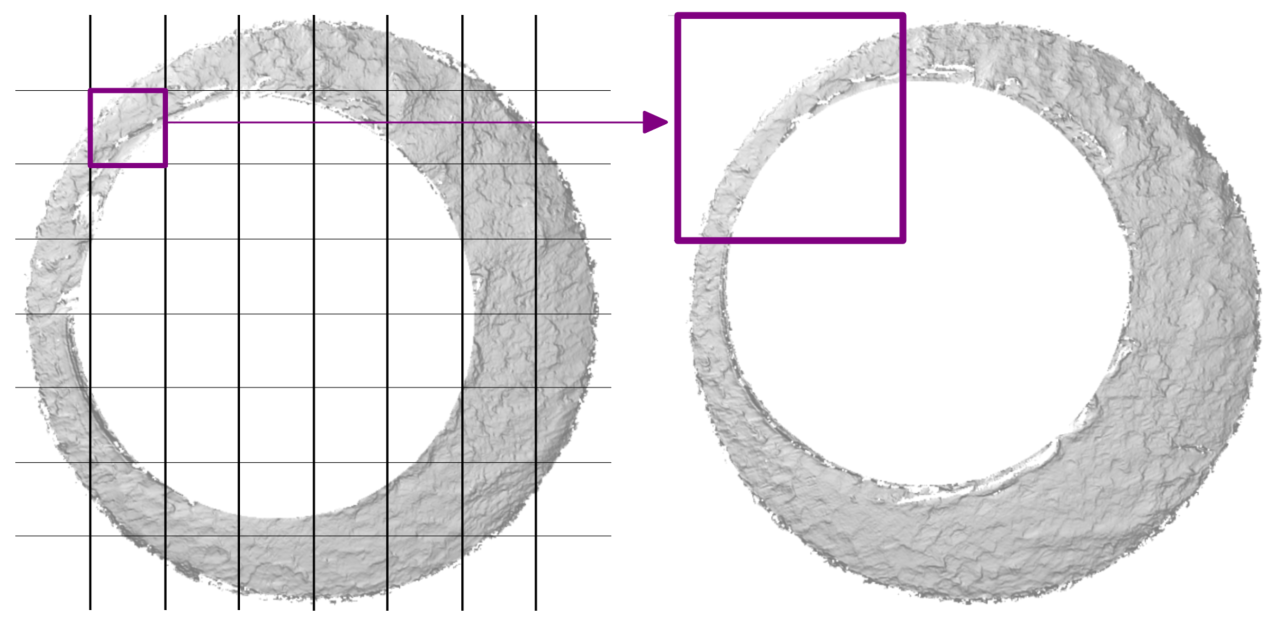
\includegraphics[width=.75\textwidth]{images/cmc_illustration} 

}

\caption{\label{fig:cmc_illustration} Illustration of comparing a cell in the reference cartridge case scan (left) to a larger region in a questioned cartridge case scan (right). Every one of the cells in the reference cartridge case is similarly paired with a region in the questioned cartridge case.  To determine the rotation at which the two cartridge cases align, the cell-region pairs are compared for various rotations of the questioned cartridge case.}\label{fig:unnamed-chunk-11}
\end{figure}
\end{Schunk}

\autoref{fig:cmc_illustration} illustrates the cell-based comparison
procedure between two cartridge case scans. The scan on the left serves
as the reference; it is divided into a grid of \(k \times k\) cells. The
cell size (and thus, the corresponding number of cells) is optimized
experimentally:

\begin{quote}
The cell size must be experimentally optimized, not too small and not
too large. Either condition may result in low correlation accuracy. For
the initial tests of 9 mm caliber cartridge cases, good correlation
results for breech face correlations were obtained using the cell sizes
ranging from (0.25 × 0.25) to (0.5 × 0.5) \(mm^2\). \citep{song_3d_2014}
\end{quote}

\begin{figure}
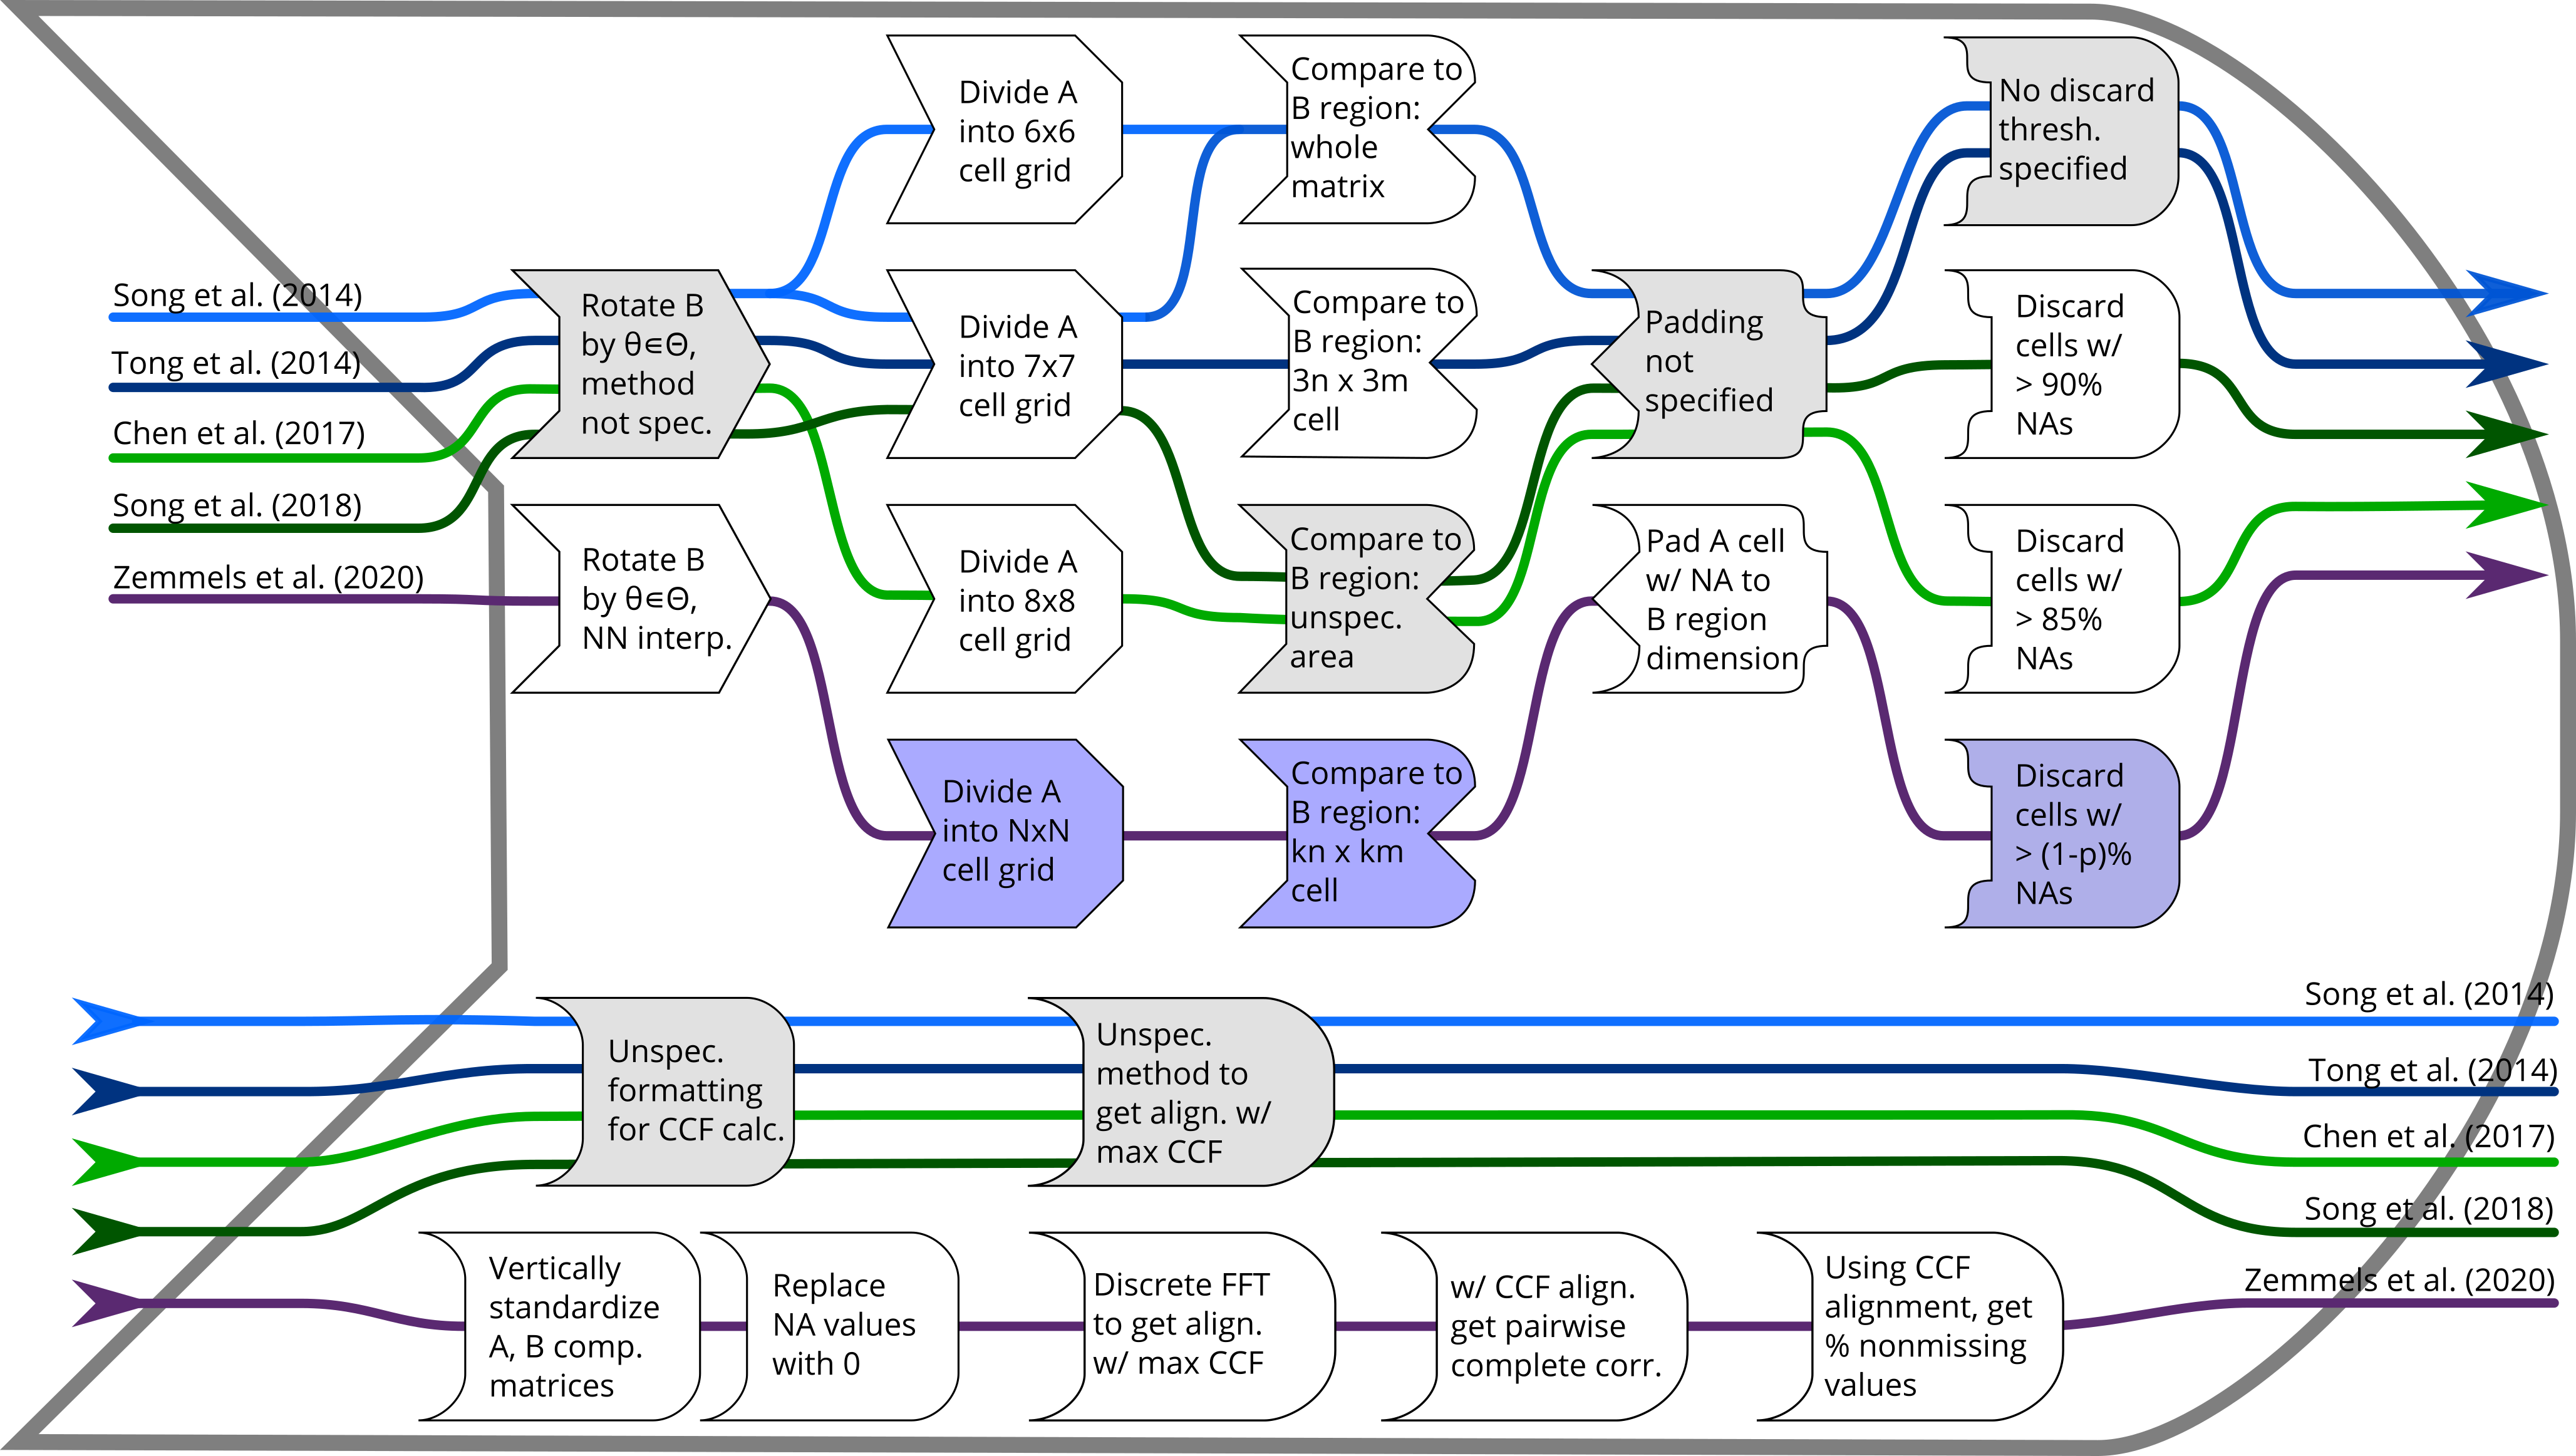
\includegraphics[width=\textwidth]{images/cmc_flow.png}
\caption{Each CMC implementation uses a slightly different procedure to obtain a similarity score between two cartridge cases. Steps which are implemented with additional user-specified parameters are shaded purple; steps which are described but without sufficient detail are shaded grey.}\label{fig:cmc-schematic}
\end{figure}

\autoref{fig:cmc-schematic} shows the steps of the correlation cell
comparison process in each of the papers as well as the \CRANpkg{cmcR}
implementation. Each cell is paired with an associated larger region in
the other scan. The absolute location of each cell and region in their
respective surface matrices remain constant. However, the scan on the
right is rotated to determine the rotation at which the two scans are
the most ``similar,'' as quantified by the
\dfn{cross-correlation function} (CCF).

For a real-valued matrices \(A\) and \(B\) of dimension \(M \times N\)
and \(P \times Q\), respectively, the cross-correlation function,
denoted \((A \star B)\) is defined as \[
(A \star B)[m,n] = \sum_{i=1}^M \sum_{j=1}^N A[i,j] B[(i + m), (j + n)],
\] where \(-(P-1) \leq m \leq M-1\) and \(-(Q-1) \leq n \leq N-1\). By
this definition, the \([m,n]\)th element of the resulting
\(M + P - 1 \times N + Q - 1\) CCF matrix quantifies the similarity
between matrices \(A\) and \(B\) for a translation of matrix \(B\) by
\(m\) pixels horizontally and \(n\) pixel vertically. The index at which
the CCF attains a maximum represents the optimal translation needed to
align \(B\) with \(A\). The CCF as defined need not be bounded between
\(-1\) and \(1\). However, it is common to normalize the CCF for
interpretability, and this is the convention adopted by the
\CRANpkg{cmcR} package.

Prior to calculating the CCF, the matrices \(A\) and \(B\) are
standardized through subtraction of their respective means and division
by their respective standard deviations. This is referred to as the
\dfn{Areal Cross-Correlation Function} (ACCF) in some CMC papers
\citep{ott_applying_2017}. A direct calculation of the CCF for breech
face scans based on the definition above is inhibitingly slow. While
computationally feasible alternatives exist, \citet{song_proposed_2013}
and other CMC papers do not specify the algorithm used to calculate the
CCF.

\citet{song_3d_2014} describe the comparison process:

\begin{quote}
CMC pairs are identified by three types of identification parameters:
the correlation value CCF\(_{\max}\), registration angle \(\theta\) and
translation distances \(x\), \(y\) with thresholds \(T_{\text{CCF}}\),
\(T_\theta\) and \(T_x, T_y\), respectively. The correlated cell pairs
are considered as CMCs when their correlation value CCF\(_{\max}\),
\(T_{\text{CCF}}\), and their registration angle \(\theta\) and \(x-y\)
registration pattern are within the thresholds \(T_\theta\), and
\(T_x, T_y\).
\end{quote}

Note, that rotating an image or breech face scan by an arbitrary angle
(other than a multiple of 90 degrees) requires interpolating new pixel
locations. A variety of interpolation schemes exist
\citep{parker_comparison_1983}, but there are no details provided in the
papers under consideration indicating which interpolation algorithm was
used. In \CRANpkg{cmcR}, surfaces matrices are rotated using a
``nearest-neighbor'' interpolation scheme \citep{imager}.

In the next section, we discuss our implementation of the cell-based
comparison procedure.

\hypertarget{implementation-of-the-correlation-cell-comparison-procedure}{%
\subsubsection{Implementation of the correlation cell comparison
procedure}\label{implementation-of-the-correlation-cell-comparison-procedure}}

All of the steps dealing with cell-based comparisons are implemented as
functions of the form \code{comparison\_*}. Similar to the
\code{preProcess\_*} functions, the \code{comparison\_*} functions can
be chained together through a sequence of pipes.

Published implementations of the CMC algorithm do not describe precisely
how the CCF is calculated. In image processing, it is common to use an
implementation based on the Fast Fourier Transform
\citep{Brown92asurvey}. This implementation leverages the
Cross-Correlation Theorem, which states that for matrices \(A\) and
\(B\), the CCF can be expressed in terms of frequency-domain pointwise
product: \[
(A \star B )[m,n]= \mathcal{F}^{-1}\left(\overline{\mathcal{F}(A)} \odot \mathcal{F}(B)\right)[m,n]
\] where \(\mathcal{F}\) and \(\mathcal{F}^{-1}\) denote the discrete
Fourier and inverse discrete Fourier transforms, respectively, and
\(\overline{\mathcal{F}(A)}\) denotes the complex conjugate
\citep{fft_brigham}. Because the product on the right-hand side is
calculated pointwise, this result allows us to trade the moving sum
computations from the definition of the CCF for two forward Fourier
transformation, a pointwise product, and an inverse Fourier
transformation. The Fast Fourier Transform (FFT) algorithm can be used
to reduce the computational load considerably. Our implementation of
this FFT-based CCF calculation is adapted from the \pkg{cartridges3D}
package \citep{cartridges3D}.

No computational shortcut comes without some tradeoffs, though, and this
FFT-based CCF calculation is no different. The FFT does not tolerate
missing values, and breech faces are not continuous surfaces -- all of
the white regions in \autoref{fig:cmc_illustration} correspond to
missing values. While it is unclear how the CCF is implemented in the
CMC papers, the \CRANpkg{cmcR} package adopts the following conventions:

\begin{itemize}
\item
  Only cells with a minimum proportion of non-missing pixels are
  assessed. This minimum threshold differs across CMC papers (15\% in
  \citet{chen_convergence_2017} vs.~10\% in
  \citet{song_estimating_2018}, as shown in
  \autoref{fig:cmc-schematic}), and is referenced but not specified in
  several other papers
  \citep{tong_fired_2014,song_3d_2014,chu_validation_2013}. The
  \code{comparison\_calcPropMissing} function computes the proportion of
  a matrix that is missing (\code{NA}-valued).
\item
  Missing values are replaced with the overall mean value when the
  FFT-based CCF is computed (using function
  \code{comparison\_replaceMissing}).
\item
  The optimal translation is determined using the FFT-based CCF (using
  \code{comparison\_fft\_ccf}).
\item
  Based on the optimal translation determined from the FFT-based CCF, we
  compute the pairwise complete CCF directly, avoiding any distortion of
  the CCF computation based on compensation for missing values (using
  function \code{comparison\_cor}).
\end{itemize}

The code below demonstrates how the \code{comparison\_allTogether}
function can be used to perform the entire cell-based comparison
procedure in one call. The comparison procedure is performed twice: once
with Fadul 1-1 considered the ``reference'' scan divided into cells that
are compared to the ``target'' scan Fadul 1-2 and again with the roles
reversed.

\begin{Schunk}
\begin{Sinput}
# Fill in most of the arguments first
comp_w_pars <- purrr::partial(.f = comparison_allTogether,
                              numCells = 64, maxMissingProp = .85)

# Then, map the remaining values to theta
kmComparisonFeatures <- purrr::map_dfr(
  seq(-30,30,by = 3),
  ~comp_w_pars(reference = fadul1.1, target = fadul1.2, theta = .))

kmComparisonFeatures_rev <- purrr::map_dfr(
  seq(-30,30,by = 3),
  ~comp_w_pars(reference = fadul1.2, target = fadul1.1, theta = .))
\end{Sinput}
\end{Schunk}

The \code{comparison\_allTogether} function consists of the following
steps wrapped into a single convenience function:

\begin{itemize}
\tightlist
\item
  \code{comparison\_cellDivision}: Divide the reference scan into cells
\item
  \code{comparison\_getTargetRegions}: Extract regions associated with
  each reference cell from the target scan
\item
  \code{comparison\_calcPropMissing}: Compute missing proportions and
  filter out cells with a proportion of missing values above the
  threshold.
\item
  \code{comparison\_standardizeHeights}: Standardize height values
\item
  \code{comparison\_replaceMissing}: Replace missing values
\item
  \code{comparison\_fft\_ccf}: Compute CCF and estimated translations
  using FFT
\item
  \code{comparison\_cor}: Compute pairwise-complete correlation between
  a reference cell and a matrix of the same size extracted from the
  associated target region
\end{itemize}

This sequence of functions are applied for a sequence of angles
\(\theta\) rotating the target scan relative to the reference scan. When
implementing the High CMC decision rule \citep{tong_improved_2015}, both
combinations of reference and target scan are examined (e.g.~A-B and
B-A).

\autoref{tab:cellCCF} shows several rows of the data frame output of the
\code{comparison\_allTogether} function for the comparison of Fadul 1-1
vs.~Fadul 1-2 considering Fadul 1-1 as the reference scan. Although a
grid of \(8 \times 8\) cells was used, there were only 26 cell-region
pairs that contained a sufficient proportion of non-missing values (15\%
in this example). The features derived from the correlation cell
procedure (CCF\(_{max}\), \(\Delta x\), \(\Delta y\), \(\theta\)) are
used as inputs to the pipelines for assessing the similarity between
scans.

\begin{Schunk}
\begin{table}

\caption{\label{tab:unnamed-chunk-13}\label{tab:cellCCF} Example of output from correlation cell comparison procedure between Fadul 1-1 and Fadul 1-2 rotated by -24 degrees. Due to the large proportion of missing values that are replaced to compute the FFT-based correlation, the pairwise-complete correlation is most often greater than the FFT-based correlation.}
\centering
\begin{tabular}[t]{|cccrrr|}
\toprule
Cell Index & Pairwise-comp. corr. & FFT-based corr. & $\Delta$x & $\Delta$y & $\theta$\\
\midrule
\cellcolor{lightgray}{1, 2} & \cellcolor{lightgray}{0.630} & \cellcolor{lightgray}{0.214} & \cellcolor{lightgray}{31} & \cellcolor{lightgray}{22} & \cellcolor{lightgray}{-24}\\
1, 3 & 0.673 & 0.295 & -1 & 11 & -24\\
\cellcolor{lightgray}{1, 4} & \cellcolor{lightgray}{0.634} & \cellcolor{lightgray}{0.255} & \cellcolor{lightgray}{-2} & \cellcolor{lightgray}{7} & \cellcolor{lightgray}{-24}\\
1, 5 & 0.525 & 0.248 & -2 & 7 & -24\\
\cellcolor{lightgray}{1, 6} & \cellcolor{lightgray}{0.658} & \cellcolor{lightgray}{0.294} & \cellcolor{lightgray}{-1} & \cellcolor{lightgray}{7} & \cellcolor{lightgray}{-24}\\
\bottomrule
\end{tabular}
\end{table}

\end{Schunk}

\hypertarget{decision-rule}{%
\subsection{Decision Rule}\label{decision-rule}}

For each cell on the reference scan, a set of rotation angles \(\theta\)
with associated translations \((\Delta x, \Delta y)\) and
cross-correlation values are calculated. These sets need to be
aggregated into a single consensus decision. Here, we describe the two
pipelines implemented in the \CRANpkg{cmcR} package: the original
decision rule described in \citet{song_3d_2014} and the High CMC
decision rule proposed in \citep{tong_improved_2015}.

The idea of a consensus decision is based on the assumption that a
matching pair of cartridge cases will have similar translation and
rotation values for all of the cells, while a non-matching pair of
cartridge cases will exhibit a variety of different translation and
rotation values without showing a particular pattern.

The first step in any CMC decision process is therefore to obtain a
consensus estimate of \(x, y, \theta\). Where the various CMC decision
rules principally differ is in how they identify a ``consensus'' among
the estimated \(x,y, \theta\) values.

\hypertarget{originalMethod}{%
\subsubsection{The Original CMC decision rule}\label{originalMethod}}

This section briefly describes the decision rule used in the first CMC
paper \citep{song_proposed_2013}. For a thorough explanation of the
procedure, refer to the
\href{https://csafe-isu.github.io/cmcR/articles/decisionRuleDescription.html}{CMC
Decision Rule Description} vignette in the \CRANpkg{cmcR} package.

Let \(x_i, y_i, \theta_i\) denote the translation and rotation
parameters which produce the highest CCF for the alignment of
cell-region pair \(i\), \(i = 1,...,n\) where \(n\) is the total number
of cell-region pairs containing a sufficient proportion of non-missing
values.

\citet{song_proposed_2013} propose the median as a consensus
\((x_{\text{ref}}, y_{\text{ref}}, \theta_{\text{ref}})\) across the
cell-region pairs for a particular cartridge case pair comparison. Then,
the distances between the consensus values and the values for each cell
comparison are assessed to determine whether the values are within a
specified distance of the consensus, as determined by three threshold
parameters \(T_{x}, T_{y}, T_\theta, T_{\text{CCF}}\).

A cell-region pair \(i\) is declared a match if all of the following
conditions hold:

\begin{eqnarray}\label{eq:original}
|x_i - x_{\text{ref}}| &\leq& T_{x} \\ \nonumber
|y_i - y_{\text{ref}}| &\leq& T_{y} \\ \nonumber
|\theta_i - \theta_{\text{ref}}| &\leq& T_{\theta} \\ \nonumber
\text{CCF}_{\max,i} &\geq& T_{\text{CCF}}.
\end{eqnarray}

The CMC count is then defined as the number of matching cell-region
pairs (out of \(n\)).

\citet{song_3d_2014} indicate that these thresholds need to be
determined experimentally. There is little consensus on an optimal set
of thresholds and no discussion of the sensitivity of proposed pipelines
to different threshold choices across CMC papers. As such, there is
little known about the effectiveness of the any CMC pipeline to
``out-of-bag'' samples.

\autoref{tab:thresholdTable} summarizes the thresholds used in various
CMC papers.

\begin{table}[ht]
\centering
\begin{tabular}{|lrrr|}
\hline
Paper & Translation $T_x, T_y$ & Rotation $\theta$ & CCF$_{\max}$ \\
& (in pixels) & (in degrees) \\
\hline
\cellcolor{lightgray}{\citet{song_3d_2014}} & \cellcolor{lightgray}{20} &
\cellcolor{lightgray}{6} & \cellcolor{lightgray}{.60} \\

\citet{tong_fired_2014} & 30 & 3 & .25 \\

\cellcolor{lightgray}{\citet{tong_improved_2015}} & \cellcolor{lightgray}{15} &
\cellcolor{lightgray}{3} & \cellcolor{lightgray}{.55} \\

\citet{chen_convergence_2017} & 20 & 3 & .40 \\

\cellcolor{lightgray}{\citet{song_estimating_2018}} & \cellcolor{lightgray}{20} &
\cellcolor{lightgray}{6} & \cellcolor{lightgray}{.50}\\
\hline
\end{tabular}
\caption{Different thresholds for translation, rotation, and CCF$_{\max}$ are used across different papers. The range in CCF$_{\max}$ is particularly notable. There is currently no principled approach to determining these thresholds. Instead, thresholds seem to be chosen by authors through experimentation and selecting thresholds that provide promising results.}
\label{tab:thresholdTable}
\end{table}

Unlike the original CMC pipeline, the High CMC decision rule considers
multiple rotations for each cell-region pair.

\hypertarget{highCMCMethod}{%
\subsubsection{The High CMC decision rule}\label{highCMCMethod}}

For the High CMC decision rule, comparisons between two scans are
performed in both directions, i.e.~each scan takes on the role of the
reference scan that is partitioned into a grid of cells.
\citet{tong_improved_2015} claim that in the original decision rule,
some matching cell-region pairs ``may be mistakenly excluded from the
CMC count'' because they attain the largest CCF value at a rotation
value outside the range allowed by \(T_\theta\) ``by chance.''

To combat this, \citet{tong_improved_2015} introduce consensus values
across all cell-region pairs for each rotation angle \(\theta\) and
calcluate a \(\theta\) dependent CMC count as the sum of matches
observed. A match is defined, as previously if a cell-region pair \(i\)
fulfills the following three conditions:

\begin{eqnarray}\label{eqn:high-cmc}
|x_{i,\theta} - x_{ref,\theta}| &\leq& T_x \\ \nonumber
|y_{i,\theta} - y_{ref,\theta}| &\leq& T_y \\ \nonumber
\text{CCF}_{i,\theta} &\geq& T_{\text{CCF}}.
\end{eqnarray}

The \(\theta\)-dependent CMC count, CMC\(_\theta\), is then defined as
the sum of matching cell-region pairs.

\citet{tong_improved_2015} assert that for a truly matching cartridge
case pair, the relationship between \(\theta\) and CMC\(_\theta\) should
exhibit a ``prominent peak'' near the true rotation value at which the
pair aligns. In contrast, truly non-matching pairs should exhibit a
``relatively flat and random {[}\ldots{]} pattern.''

To determine whether a ``prominent peak'' exists in the relationship
between \(\theta\) and CMC\(_\theta\), \citet{tong_improved_2015}
introduce the ``angular range'' \(R (\tau)\) as an interval of rotation
angles covering high CMC\(_\theta\) values. Here, \(\tau\) represents
another threshold value that determines the angular range as the
interval of angles between
\(\arg \min_\theta CMC_\theta > CMC_{\text{max}} - \tau\) and and
\(\arg \max_\theta CMC_\theta < CMC_{\text{max}} - \tau\), where
\(CMC_{\text{max}}\) is defined as the maximum of CMC\(_\theta\) counts
across all rotation angles \(\theta\). \citet{tong_improved_2015}
suggest a value for \(\tau\) of 1 and further determine:

\begin{quote}
If the angular range of the ``high CMCs'' is within the range
\(T_\theta\), identify the CMCs for each rotation angle in this range
and combine them to give the number of CMCs for this comparison in place
of the original CMC number.
\end{quote}

If the angular range is outside the range of \(T_\theta\), we say that
the cartridge case pair ``fails'' the High CMC criteria and the original
CMC number is used. Using this definition, the High CMC decision rule
returns for any comparison of breech face scans a CMC count equal to or
higher to the original decision rule for both known matches and known
non-matches.

\hypertarget{decisionRuleImplementation}{%
\subsubsection{Implementation of decision
rules}\label{decisionRuleImplementation}}

In this section, we demonstrate the implementation of the decision rules
in \CRANpkg{cmcR} for both the original decision rule and the High CMC
decision rule. For illustrative purposes, let us consider a particular
set of thresholds: \(T_x = T_y = 20\), \(T_{\theta} = 6\), and
\(T_{\text{CCF}} = .5\) values.

Decision rules in \CRANpkg{cmcR} are implemented as functions of the
form \code{decision\_*}. In particular, the \code{decision\_CMC}
function applies both the original and High CMC decision rules\}
depending on whether a value for \(\tau\) is provided. The code below
demonstrates the use of \code{decision\_CMC} on the features
\code{kmComparisonFeatures}, extracted from the comparison of scans
Fadul 1-1 and Fadul 1-2. \code{kmComparisonFeatures\_rev} contains the
features from a comparison of Fadul 1-2 and Fadul 1-1. Addiionally, we
also compute the CMCs under both decision rules for the comparison
between the non-match pair Fadul 1-1 and Fadul 2-1 (not shown to avoid
redundancy).

\begin{Schunk}
\begin{Sinput}
kmComparison_cmcs <- kmComparisonFeatures %>% mutate(
  originalMethodClassif =
    decision_CMC(cellIndex = cellIndex, x = x, y = y, theta = theta,
                 corr = pairwiseCompCor, xThresh = 20, thetaThresh = 6,
                 corrThresh = .5),
  highCMCClassif =
    decision_CMC(cellIndex = cellIndex, x = x, y = y, theta = theta,
                 corr = pairwiseCompCor, xThresh = 20, thetaThresh = 6,
                 corrThresh = .5, tau = 1))
\end{Sinput}
\end{Schunk}

We can use the \code{cmcPlot} function to visualize CMCs and non-CMCs.
\autoref{fig:topVoteCMCPlot} shows congruent matching cells (CMCs) and
non-congruent matching cells (non-CMCs) determined under the original
decision rule in blue and red, respectively. The (red) non-CMC patches
are located in the position where the maximum CCF value in the target
scan is attained. The top row shows 17 CMCs in blue and 10 non-CMCs in
red when Fadul 1-1 is treated as the reference and Fadul 1-2 the target.
The bottom row shows the 18 CMCs and 14 non-CMCs when the roles are
reversed. There is no discussion in \citet{song_proposed_2013} about
combining the results from these two comparison directions, but
\citet{tong_improved_2015} propose using the minimum of the two CMC
counts (17 in this example).

\begin{Schunk}
\begin{figure}[htbp]

{\centering 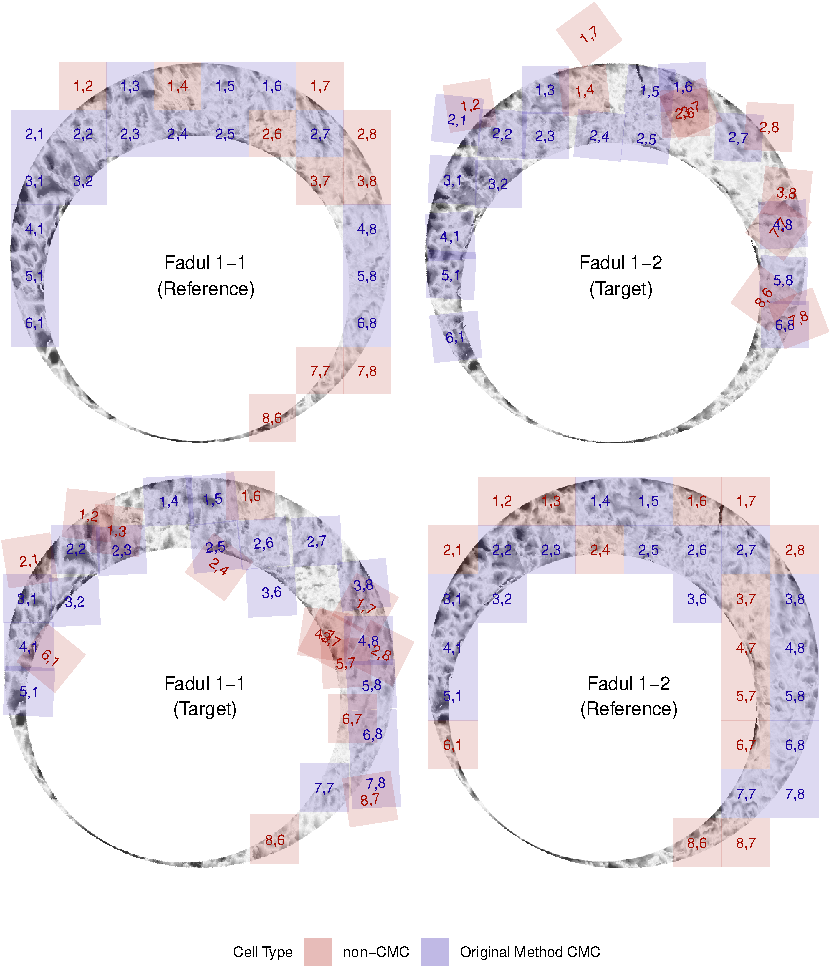
\includegraphics[width=\textwidth]{figures/kmOriginalMethod} 

}

\caption{\label{fig:topVoteCMCPlot} CMC results for the comparison between Fadul 1-1 and Fadul 1-2 using the original decision rule. The two plots in the top row show the 17 CMCs when Fadul 1-1 is treated as the ``reference" cartridge case to which Fadul 1-2 (the ``target") is compared. The second row shows the 18 CMCs when the roles are reversed. Red cells indicate where cells \emph{not} identified as congruent achieve the maximum pairwise-complete correlation across all rotations of the target scan. }\label{fig:unnamed-chunk-16}
\end{figure}
\end{Schunk}

Similarly, CMCs and non-CMCs determined under the High CMC decision rule
are shown in \autoref{fig:highCMCPlot}. Treating Fadul 1-1 and Fadul 1-2
as the reference scan yields 19 and 18 CMCs, respectively. Combining the
results as described above, the final High CMC number is 24 CMCs.

\begin{Schunk}
\begin{figure}[htbp]

{\centering 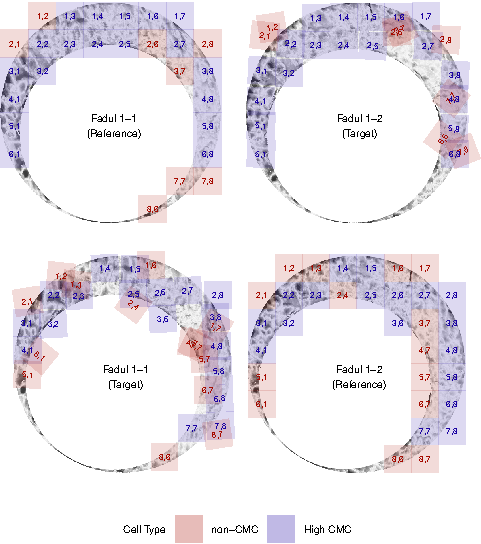
\includegraphics[width=\textwidth]{figures/kmHighCMC} 

}

\caption{\label{fig:highCMCPlot} Applying the High CMC decision rule to the comparison of Fadul 1-1 and Fadul 1-2 results in 19 CMCs when Fadul 1-1 is treated as the reference (top) and 18 CMCs when Fadul 1-2 is treated as the reference (bottom). Although the individual comparisons do not yield considerably more CMCs than under the original CMC pipeline, \citet{tong_improved_2015} indicate that the High CMCs from both comparisons are combined as the final High CMC count (each cell is counted at most once). Combining the results means that the High CMC decision rule tends to produce higher CMC counts than the original CMC pipeline. In this example, the combined High CMC count is 24 CMCs.}\label{fig:unnamed-chunk-17}
\end{figure}
\end{Schunk}

In contrast, \autoref{fig:knmCMCPlot} shows the CMC results for a
comparison between Fadul 1-1 and a known non-match scan, Fadul 2-1,
under the exact same processing conditions. Only one cell is classified
as a congruent matching cell under the original decision rule when Fadul
1-1 is the reference scan. No cells are classified as CMCs in the other
direction. While not shown, this pair fails the High CMC criteria and
thus was assigned 0 CMCs under the High CMC decision rule.

\begin{Schunk}
\begin{figure}[htbp]

{\centering 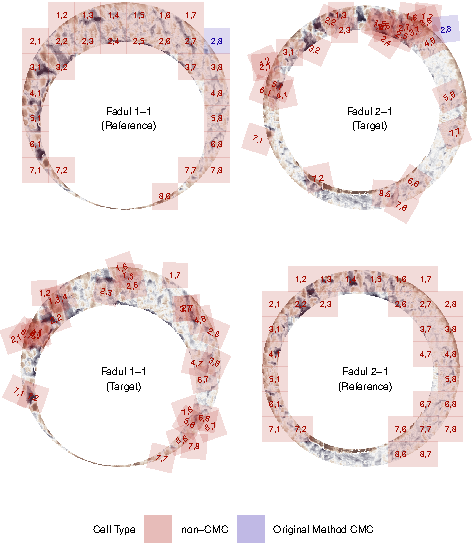
\includegraphics[width=\textwidth]{figures/knmOriginalMethod} 

}

\caption{\label{fig:knmCMCPlot} Applying both decision rules to the comparison between the non-match pair Fadul 1-1 and Fadul 2-1 results in 1 CMC under the original decision rule (shown above) and 0 CMCs under the High CMC decision rule (not shown). The seemingly random behavior of the red cells exemplifies the assumption that cells in a non-match comparison do not exhibit an observable pattern. Random chance should be the prevailing factor in classifying non-match cells as CMCs.}\label{fig:unnamed-chunk-18}
\end{figure}
\end{Schunk}

\hypertarget{ambiguities}{%
\subsection{Ambiguity in algorithmic descriptions}\label{ambiguities}}

During the implementation process we encountered various ambiguities in
the descriptions of the various CMC pipelines. In the following section
we investigate ways in which such ambiguities can be rectified by
exploring a set of reproducibility principles.

We include the preprocessing and cell-based comparison procedures as
part of the CMC methodology to emphasize how much the final results
depend on decisions made in these first two steps. The preprocessing and
cell-based comparison procedures are discussed only briefly, if at all,
in \citet{song_3d_2014}, \citet{tong_fired_2014},
\citet{tong_improved_2015}, or \citet{chen_convergence_2017}, yet, the
results reported often indicate a sensitivity to these procedures. An
actual sensitivity analysis of proposed CMC pipelines has yet to be
published. Left unchecked, this can lead to results that are difficult
to generalize to new data.

Apart from the CMC pipelines' generalizability, we also simply do not
know how the proposed pipelines are implemented. Ambiguities in the
pipelines range from minor implicit parameter choices (e.g., the
convergence criteria for the robust Gaussian regression filter
\citep{brinkman_bodschwinna_2003}) to procedures that fundamentally
change how similarity features are extracted and compared (e.g., how the
cross-correlation is calculated). As discussed in the
\protect\hyperlink{intro}{introduction}, this is an issue that pervades
computational research for which only verbal descriptions of algorithms
are provided. The only solution to such ambiguity is to enumerate,
implement, and pare-down the possible choices that could have been made
to arrive to published results. Unsurprisingly, this process takes a
considerable amount of time and resources that would be better spent
furthering the state of the field.

In the next section, we describe the process of resolving these
ambiguities in the CMC pipeline descriptions. In doing so, we abstract a
set of principles by which pipelines and results can be rendered both
computationally reproducible and more thoroughly understood.

\hypertarget{investigation}{%
\section{Investigation of cell-based forensic pattern matching
pipelines}\label{investigation}}

As described in the \protect\hyperlink{initialData}{initial data}
section, the set of cartridge case scans from
\citet{fadul_empirical_2011} is commonly used to compare the performance
of various classification methods
\citep{song_3d_2014, tong_improved_2015, chen_convergence_2017}. This
set consists of 40 cartridge cases and 780 total comparisons: 63 known
match comparisons and 717 known non-match comparisons. Scans of each
breech face impression were taken with a Nanofocus Confocal Light
Microscope at 10 fold magnification for a nominal lateral resolution of
3.125 microns per pixel and published as part of NBTRD \citep{nbtrd}.
While the exact procedures by which these scans were processed in the
original CMC papers are unavailable, these 3D topographic surface images
provide the basis of the comparison between the implementation provided
in the \CRANpkg{cmcR} package and published results. However,
justification for any differences will ultimately involve educated
hypothesization due to the closed-source nature of the original
implementations.

For any cartridge case pair, the number of CMCs can be determined under
the original decision rule and the High CMC decision rule described in
the \protect\hyperlink{implementation}{implementation} section. We have
applied our implementation of these two methods to the 780 cartridge
case pairs available in the \citet{fadul_empirical_2011} data set under
a variety of processing conditions to determine which conditions yield
the best results while also matching the published results. Perfect
identification of all matching and non-matching pairs corresponds to
choosing a minimum CMC count threshold that separates the distributions
of the matching and non-matching CMC counts. A CMC count threshold of 6
CMCs is generally accepted as the threshold in the published papers
\citep{tong_improved_2015,song_estimating_2018,song_proposed_2013}.
However, this threshold has been shown to not generalize well to all
proposed methods and cartridge case data sets
\citep{chen_convergence_2017}. In this section, we demonstrate that the
ambiguities in the \href{cmcMethod}{CMC pipeline descriptions} and lack
of guidance in the choice of parameter settings propagate through the
algorithm and produce highly variable results. Additionally, wildly
different parameter settings are used by the same group of authors
across different papers as shown in \autoref{tab:thresholdTable}.

In the next section we focus on a discussion of the sensitivity of some
of the pipeline's parameters. This presentation is far from exhaustive:
we primarily focus on the factors contributing to the most variable
results. As a consequence of this investigation we have developed a set
of principles designed to reduce the need for brute-force searches
across parameter settings when re-implementing algorithms without
accompanying code. Adherence to these principles yields not only
computationally reproducible results, but also improves a reader's
understanding of a proposed pipeline.

\hypertarget{communicating-a-methods-sensitivity-to-processing-conditions}{%
\subsection{Communicating a method's sensitivity to processing
conditions}\label{communicating-a-methods-sensitivity-to-processing-conditions}}

Choosing threshold values \(T_x, T_y, T_\theta, T_{\text{CCF}}\) for
translation, rotation and maximum cross-correlation is crucial in
declaring a particular cell-region pair ``congruent''. Many different
combinations of these thresholds yield perfect separation between the
matching and non-matching CMC count distributions. In situations where
ground truth is known, such as in the example of the Fadul data here, we
can use the ratio \(r\) of between- and within-group variability as an
additional statistic to measure separation between CMC counts of known
matches and known non-matches. Let C\(_{ij}\) denote the CMC count
assigned to the \(j\)th cartridge case pair, \(j = 1,...,n_i\),
\(n_1 = 63, n_2 = 717\), from the \(i\)th group, \(i = 1,2\)
representing matches and non-matches, respectively. For each set of
thresholds we calculate the \textbf{Variance Ratio} \(r\) as: \[
r = r\left(T_x, T_y, T_\theta, T_{\text{CCF}}\right) = \frac{\sum_{i=1}^2 \left(\overline{C}_{i.} - \overline{C}_{..}\right)^2}{\sum_{i=1}^2 \frac{1}{n_i - 1}\sum_{j=1}^{n_i} \left(C_{ij} - \overline{C}_{i.}\right)^2}
\] where \(\overline{C}_{i.}\) denotes the within-group CMC count
average and \(\overline{C}_{..}\) denotes the grand CMC count average.
Greater separation between and less variability within the match and
non-match CMC count distributions yields larger \(r\) values. Larger
values of \(r\) are therefore indicative of greater separation between
the groups.

\autoref{fig:decisionRuleSensitivity_comparison} shows results for the
original decision rule and the High CMC decision rule for a parameter
setting of \(T_{\Delta x} = 20 = T_{\Delta y}\) pixels,
\(T_{\text{CCF}} = .5\), and \(T_{\theta} = 6\). Both decision rules
result in separated CMC count distributions for known matches and known
non-matches corresponding to an AUC of 1.00. However, the High CMC
decision rule yields a larger separation between the known match and
known non-match distributions as evidenced by the considerably larger
variance ratio \(r\).

\begin{Schunk}
\begin{figure}[htbp]

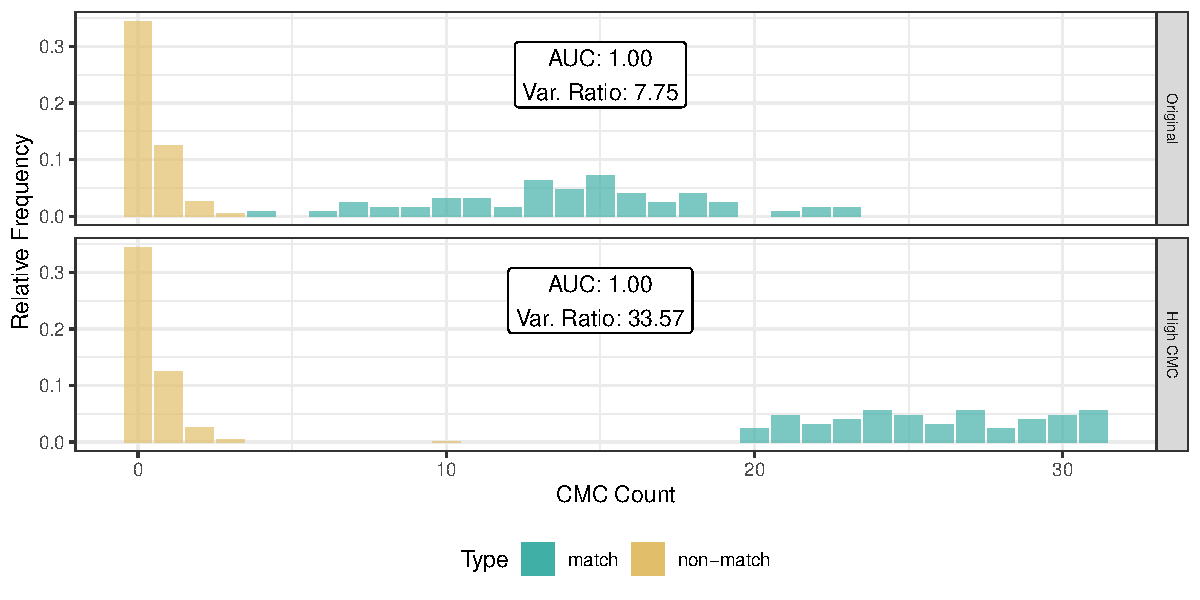
\includegraphics[width=\textwidth]{figures/cmcr-unnamed-chunk-19-1} \hfill{}

\caption{\label{fig:decisionRuleSensitivity_comparison} CMC count relative frequencies under the original decision rule and the High CMC decision rule for $T_{\Delta x} = 20 = T_{\Delta y}$ pixels, $T_{\text{CCF}} = .5$, and $T_{\theta} = 6$ degrees. AUC $= 1.00$ corresponds to perfect separation of the match and non-match CMC count distributions. We can see that, for this set of processing parameters, the High CMC decision rule yields higher CMC counts for known matches that the original decision rule while known non-matches have the same distribution under both methods.}\label{fig:unnamed-chunk-19}
\end{figure}
\end{Schunk}

We consider five dimensions that have a demonstrable impact on the
effectiveness of the CMC pipeline. These include:

\begin{itemize}
\item the decision rule (original or High CMC) used,

\item whether the global trend is removed during preprocessing, and

\item choice of congruency thresholds: translation $T_x, T_y$, rotation $T_\theta$, and cross-correlation $T_{\text{CCF}}$.
\end{itemize}

Choosing a single parameter setting resulting in perfect identification
is not enough to generally understand the algorithm. Instead, we use the
variance ratio \(r\) to identify promising ranges of parameters.
\autoref{fig:cmc_sensitivityScatter} shows the value of the variance
ratio under various settings. We see that the High CMC decision rule
yields better separation than the original decision rule under any
parameter setting. Highest variance ratios, however, are achieved for
thresholds \(T_x, T_y \in [10,20]\), \(T_\theta = 6\), and
\(T_{\text{CCF}} \in [.4,.5]\). Interestingly, as seen in
\autoref{tab:thresholdTable}, only the parameters for the High CMC
decision rule discussed in \citet{song_estimating_2018} fall into these
ranges.

\begin{Schunk}
\begin{figure}[htbp]

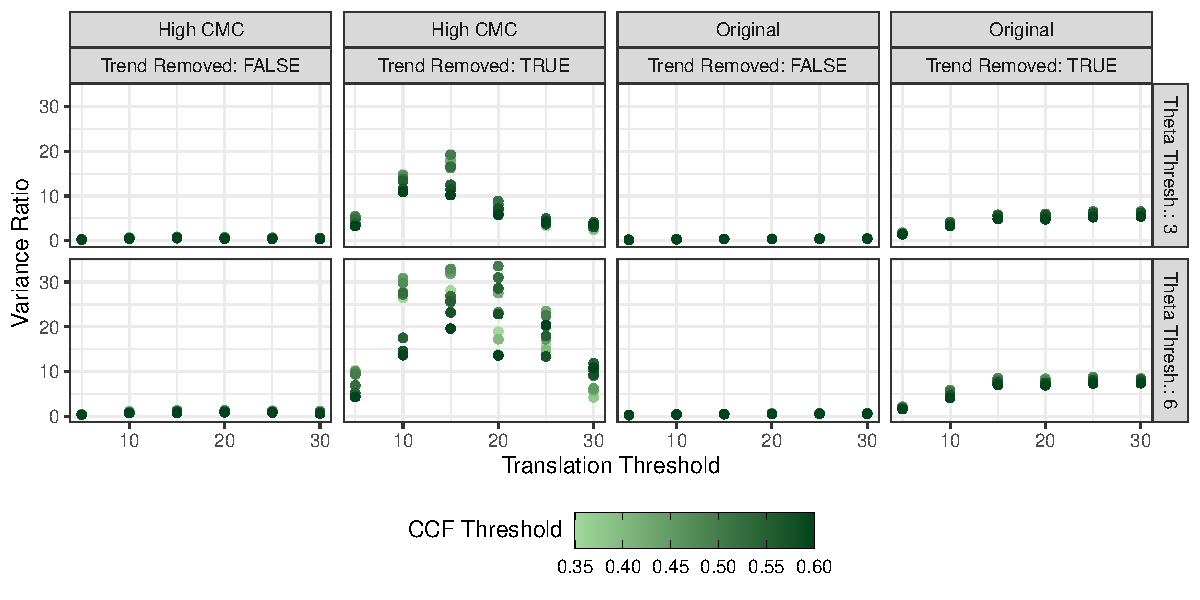
\includegraphics[width=\textwidth]{figures/cmcr-unnamed-chunk-20-1} \hfill{}

\caption{\label{fig:cmc_sensitivityScatter} Variance ratios under are plotted for different parameter settings. High variance ratios are indicative of a a good separation between CMC counts for known matching pairs and known-non matching pairs. The High CMC decision rule generally performs better than the original decision rule. Removing the trend during preprocessing, even though not explicitly described as a preprocessing step in the CMC papers, has a major impact on the effectiveness of the CMC pipeline. In this setting, translation thresholds $T_x, T_y \in [15,20]$, a rotation threshold $T_\theta = 6$, and a CCF threshold $T_{\text{CCF}} \in [.4,5]$ lead to a separation of results. }\label{fig:unnamed-chunk-20}
\end{figure}
\end{Schunk}

As shown in \autoref{fig:cmc_sensitivityScatter}, de-trending
breech-scans in the preprocessing stage emerges as a very impactful step
to achieve good algorithmic results. This step is not explicitly
mentioned in the written-word descriptions of the algorithm in either of
the papers by \citet{song_proposed_2013}, \citet{tong_fired_2014},
\citet{tong_improved_2015}, \citet{chen_convergence_2017}, or
\citet{song_estimating_2018}, though it appears from their examples that
it was used in the process. This highlights, yet again, the dangers of
only providing verbal instructions in lieu of code.
\autoref{fig:cmc_sensitivityScatter} also shows us the benefits of
breaking a pipeline up into modularized steps for an algorithmic
analysis. We will expand upon this in the next section.

\autoref{fig:cmc_varRatioComparison} shows variance ratio values based
on results presented in various CMC papers using data from
\citet{fadul_empirical_2011} and \citet{weller_2012}. Note that the
breech face impression region were identified manually for the
\citet{weller_2012} dataset using the FiX3P software (accessible here:\}
\url{https://github.com/talenfisher/fix3p}). These processed data are
available upon request due to their size. We can see that the High CMC
decision rule yields higher variance ratio values than the original
decision rule. However, as discussed previously, it is difficult to
justify differences in these values because the various papers different
preprocessing procedures and parameters (e.g., see
\autoref{tab:thresholdTable}). The last two rows show the largest
variance ratio values for the original and High CMC decision rules based
on the grid search summarized in \autoref{fig:cmc_sensitivityScatter}.
In particular, the highest variance ratio value for the original
decision rule is associated with translation thresholds
\(T_x = T_y = 25\), rotation threshold \(T_\theta = 6\), and correlation
threshold \(T_{\text{CCF}} = .45\). The highest variance ratio value for
the High CMC decision rule is associated with translation thresholds
\(T_x = T_y = 20\), rotation threshold \(T_\theta = 6\), and correlation
threshold \(T_{\text{CCF}} = .5\). This demonstrates that the
implementation provided in \CRANpkg{cmcR} yields comparable results to
previous CMC papers.

\begin{Schunk}
\begin{figure}[htbp]

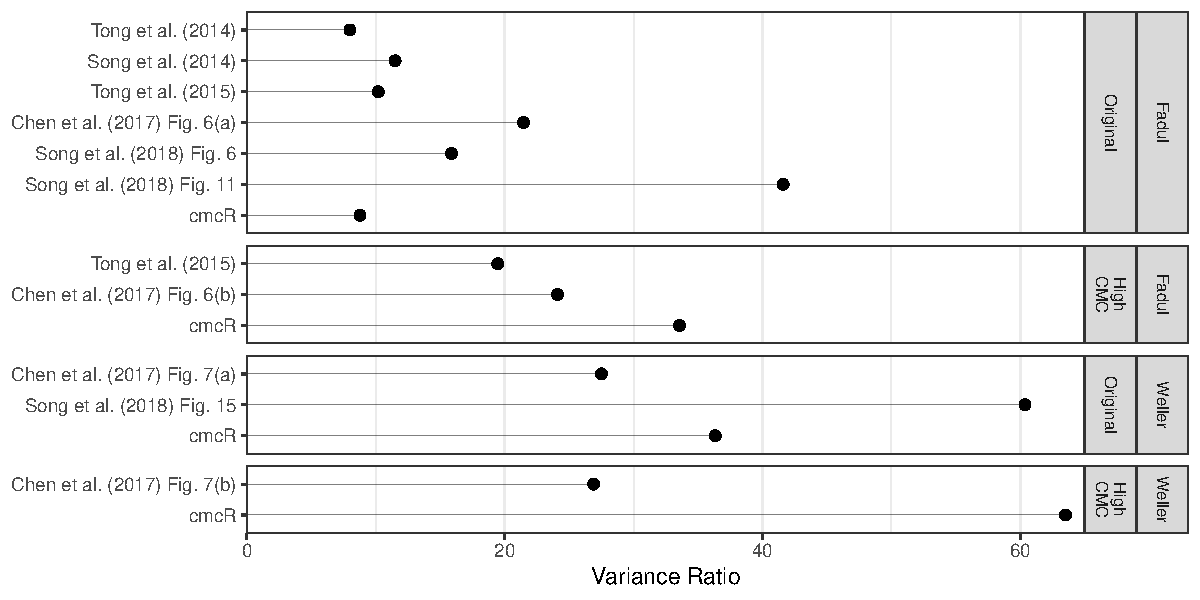
\includegraphics[width=\textwidth]{figures/cmcr-unnamed-chunk-21-1} \hfill{}

\caption{\label{fig:cmc_varRatioComparison} Variance ratios based on results reported in various CMC papers. The High CMC decision rule tends to outperform the original decision rule. However, it should be emphasized that each paper uses very different processing and parameter settings (e.g., the thresholds used are summarized in \autoref{tab:thresholdTable}) meaning the results are difficult to compare. The values labeled "cmcR" show the largest variance ratio values for the original and High CMC decision rules based on a limited grid search. These results indicate that the CMC pipeline implementation provided in \CRANpkg{cmcR} yields comparable results to previous CMC papers.}\label{fig:unnamed-chunk-21}
\end{figure}
\end{Schunk}

\hypertarget{discussion}{%
\section{Discussion and Conclusion}\label{discussion}}

Reproducibility is an indispensable component of scientific validity
\citep{goodman_what_2016}. In this paper, we demonstrate at least three
ways reproducibility can go awry: ambiguity in procedural
implementation, missing or incomplete data, and missing or incomplete
code. The papers which present the CMC algorithm provide human-friendly
descriptions of the CMC pipeline, but fail to provide sufficient details
for an outside group to easily reproduce the work. Our contribution to
the CMC literature is the open-source implementation, which removes any
descriptive ambiguity in the human-friendly descriptions in the original
papers; we provide more detailed, hardware-friendly code which serves as
a companion to the original papers. While we have largely succeeded in
reproducing the published results of the CMC algorithm, some uncertainty
remains. It is possible that our pipeline may not sufficiently reproduce
the original authors' results on an external data set, which is an
important assessment for any computational algorithm
\citep{vanderplasComparisonThreeSimilarity2020}. It is worth considering
the obstacles we encountered during the implementation, because they are
common when attempting to recreate the computational steps in a paper
published without code, pseudocode, or data, as described in
\ref{reprod-defn}.

Initially, we began by comparing the published CMC papers to develop the
preprocessing and decision rule charts shown in Figures
\ref{fig:preprocessing-schematic} and \ref{fig:processingPipeline}. The
most troublesome portion of the process was that we had to replicate the
manual preprocessing of the scans before the algorithmic steps were
applied: this step in particular could have been easily avoided had the
authors shared the manually processed data along with their paper. There
were additionally some difficulties with the availability of band pass
filters -- the R equivalents of these filters may or may not precisely
emulate the MatLab filters which were applied in the CMC papers,
however, we think it likely that the primary issue with reproducing this
step of the pipeline is in the manual data cleaning component.

While none of these factors are unique to the CMC algorithm, what is
unique is the particular combination of an algorithm with many
parameters that is extremely sensitive to the parameter settings and the
gravity of the material the algorithm is intended to process. The
extreme sensitivity of the CMC algorithm to parameter settings is
problematic precisely because the data processed by the algorithm is
eventually intended to support forensic examiner decision making and
eventually, courtroom testimony. If many parameter settings are valid
but only a narrow range lead to the same conclusion, it is entirely
possible that witnesses for the prosecution and defense may come to
different conclusions. In order to prevent such misunderstandings, it is
not enough to have guidelines for parameter settings and/or a
sensitivity study -- it is also necessary to standardize the specific
computer code, because the parameter values are only useful within the
context of a single software package or pipeline. The papers presenting
the CMC algorithm are not sufficient to ensure this level of
reproducibility in the results, even though the papers themselves
provide a solid foundation. Rather, the CMC algorithm itself highlights
the importance of open software and full reproducibility: the algorithm
is not useful in the context of the wider problem it is hoping to solve
unless there is a software implementation and documented results on data
provided for general consumption. A completely reproducible paper
requires not only algorithm descriptions, but also open-source code,
initial and any manually processed data, documentation detailing
language/package versions, random seeds, metadata, and other essential
details.

While this example is compelling, it is far from unique: some journals
have adopted policies encouraging or requiring that authors provide code
and data sufficient to reproduce the statistical analyses, with the goal
of building a ``culture of reproducibility'' in their respective fields
\citep{peng_reproducible_2009, peng_reproducible_2011, stodden_toward_2013}.
Peer-review and scientific progress in the truest sense requires that
\emph{all} pre-processed data, code, and results be made openly
available \citep{kwongAlgorithmSaysYou2017, desaiTrustVerifyGuide2017}.
Our experience with the CMC algorithm suggests that these standards
should be adopted by the forensic science community, leveraging
open-source ecosystems like R and software sharing platforms such as
Github.

The modular approach used in \CRANpkg{cmcR} makes it easier to describe
the algorithm, easier to write the code, modify and improve the method,
and show that the improvement has a noticeable impact on the results.
The modularization creates an explicit framework for assessment of the
utility and effectiveness of each piece of the algorithm, and allows us
to specifically manipulate each step independently, while monitoring the
downstream impact on the results. Additionally, it allows future
collaborators to improve on pieces of the pipeline, adding additional
options and improving the method without having to re-invent the wheel.
Indeed, re-implementing steps of the pipeline is at best a useful
academic exercise and at worst a waste of time and resources that could
be spent actually improving the pipeline. These principles of open,
accessible, interoperable code are also critical for a fair (in the
legal sense) justice system: the defense has access to the code to
understand the evidence against them, lawyers and examiners can assess
the utility of the analysis method, and judges can determine whether a
method is admissible in court. Transparent and intuitive open-source
algorithms, such as \CRANpkg{cmcR}, should be considered the gold
standard in allowing the forensic science community to validate a
pipeline. We intend the \CRANpkg{cmcR} package to serve as a flexible,
easy-to-use foundation upon which improvements to the CMC pipeline can
be developed.

We firmly believe that the forensic community does not go only halfway,
trading a subjective, human black box for objective, proprietary
algorithms that are similarly opaque and unauditable. In addition to the
benefits to forensic examiners who may use CMC algorithms to support
decisions made about evidence, the full reproducibility standard
benefits the wider research community. Open, fully reproducible packages
like \CRANpkg{cmcR} allow research groups to make incremental changes,
compare different approaches, and accelerate the pace of research and
development.

\hypertarget{acknowledgement}{%
\section{Acknowledgement}\label{acknowledgement}}

This work was partially funded by the Center for Statistics and
Applications in Forensic Evidence (CSAFE) through Cooperative Agreement
70NANB20H019 between NIST and Iowa State University, which includes
activities carried out at Carnegie Mellon University, Duke University,
University of California Irvine, University of Virginia, West Virginia
University, University of Pennsylvania, Swarthmore College and
University of Nebraska, Lincoln.

We greatly appreciate the constructive feedback from the two anonymous
reviewers. Special thanks also to all the developers and open-source
contributors of R \citep{R}, knitr \citep{knitr1, knitr2}, rticles
\citep{rticles}, and the tidyverse \citep{tidyverse}, without whom this
project would not have been possible.

\hypertarget{computational-details}{%
\section{Computational details}\label{computational-details}}

\begin{Schunk}
\begin{Sinput}
sessionInfo()
\end{Sinput}
\begin{Soutput}
#> R version 4.1.1 (2021-08-10)
#> Platform: x86_64-w64-mingw32/x64 (64-bit)
#> Running under: Windows 10 x64 (build 22000)
#> 
#> Matrix products: default
#> 
#> locale:
#> [1] LC_COLLATE=English_United States.1252 
#> [2] LC_CTYPE=English_United States.1252   
#> [3] LC_MONETARY=English_United States.1252
#> [4] LC_NUMERIC=C                          
#> [5] LC_TIME=English_United States.1252    
#> 
#> attached base packages:
#> [1] stats     graphics  grDevices utils     datasets  methods   base     
#> 
#> other attached packages:
#>  [1] patchwork_1.1.1 rgl_0.107.14    x3ptools_0.0.3  forcats_0.5.1  
#>  [5] stringr_1.4.0   dplyr_1.0.7     purrr_0.3.4     readr_2.0.1    
#>  [9] tidyr_1.1.3     tibble_3.1.4    ggplot2_3.3.5   tidyverse_1.3.1
#> [13] cmcR_0.1.6     
#> 
#> loaded via a namespace (and not attached):
#>  [1] matrixStats_0.60.1 fs_1.5.0           lubridate_1.7.10   webshot_0.5.2     
#>  [5] httr_1.4.2         tools_4.1.1        backports_1.2.1    utf8_1.2.2        
#>  [9] R6_2.5.1           DBI_1.1.1          colorspace_2.0-2   withr_2.4.2       
#> [13] readbitmap_0.1.5   tidyselect_1.1.1   gridExtra_2.3      compiler_4.1.1    
#> [17] cli_3.0.1          rvest_1.0.1        quantreg_5.86      SparseM_1.81      
#> [21] xml2_1.3.2         labeling_0.4.2     scales_1.1.1       systemfonts_1.0.2 
#> [25] digest_0.6.27      tiff_0.1-8         svglite_2.0.0      rmarkdown_2.11    
#> [29] rticles_0.21       jpeg_0.1-9         pkgconfig_2.0.3    htmltools_0.5.2   
#> [33] dbplyr_2.1.1       fastmap_1.1.0      htmlwidgets_1.5.4  rlang_0.4.11      
#> [37] readxl_1.3.1       rstudioapi_0.13    generics_0.1.1     farver_2.1.0      
#> [41] zoo_1.8-9          jsonlite_1.7.2     magrittr_2.0.1     kableExtra_1.3.4  
#> [45] Matrix_1.3-4       Rcpp_1.0.7         munsell_0.5.0      fansi_0.5.0       
#> [49] ggnewscale_0.4.5   lifecycle_1.0.1    stringi_1.7.4      yaml_2.2.1        
#> [53] MASS_7.3-54        grid_4.1.1         crayon_1.4.2       lattice_0.20-44   
#> [57] cowplot_1.1.1      haven_2.4.3        hms_1.1.0          knitr_1.34        
#> [61] pillar_1.6.4       igraph_1.2.6       codetools_0.2-18   imager_0.42.10    
#> [65] reprex_2.0.1       glue_1.4.2         evaluate_0.14      bmp_0.3           
#> [69] modelr_0.1.8       vctrs_0.3.8        png_0.1-7          tzdb_0.1.2        
#> [73] MatrixModels_0.5-0 cellranger_1.1.0   gtable_0.3.0       assertthat_0.2.1  
#> [77] xfun_0.25          broom_0.7.9        pracma_2.3.3       viridisLite_0.4.0 
#> [81] conquer_1.0.2      ellipsis_0.3.2
\end{Soutput}
\end{Schunk}

\bibliography{zemmels-vanderplas-hofmann}


\address{%
Joseph Zemmels\\
Center for Statistics and Applications in Forensic Evidence\\%
Department of Statistics\\ Iowa State University\\ 2438 Osborn
Drive\\ Ames, IA 50011\\
%
%
%
\href{mailto:jzemmels@iastate.edu}{\nolinkurl{jzemmels@iastate.edu}}%
}

\address{%
Susan VanderPlas\\
University of Nebraska - Lincoln\\%
Department of Statistics\\ 340 Hardin Hall North Wing\\ Lincoln, NE
68583\\
%
%
%
\href{mailto:susan.vanderplas@unl.edu}{\nolinkurl{susan.vanderplas@unl.edu}}%
}

\address{%
Heike Hofmann\\
Center for Statistics and Applications in Forensic Evidence\\%
Department of Statistics\\ Iowa State University\\ 2438 Osborn
Drive\\ Ames, IA 50011\\
%
%
%
\href{mailto:hofmann@iastate.edu}{\nolinkurl{hofmann@iastate.edu}}%
}
